\documentclass[12pt]{article}
\usepackage[portuguese]{babel}
\usepackage{natbib}
\usepackage{url}
\usepackage[utf8x]{inputenc}
\usepackage{amsmath}
\usepackage{graphicx}
\usepackage{tikz,lipsum,lmodern}
\usepackage[most]{tcolorbox}
\usepackage{parskip}
\usepackage{fancyhdr}
\usepackage{vmargin}
\usepackage{listings}
\usepackage{color}
\usepackage{float}
\usepackage{multicol}
\usepackage[T1]{fontenc}
\usepackage{lmodern}

\graphicspath{{images/}}
\setmarginsrb{3 cm}{2.5 cm}{3 cm}{2.5 cm}{1 cm}{1.5 cm}{1 cm}{1.5 cm}

%Syntax highlighting
\definecolor{dkgreen}{rgb}{0,0.6,0}
\definecolor{gray}{rgb}{0.5,0.5,0.5}
\definecolor{mauve}{rgb}{0.58,0,0.82}

\lstset{frame=tb,
  language=C,
  aboveskip=3mm,
  belowskip=3mm,
  showstringspaces=false,
  columns=flexible,
  basicstyle={\small\ttfamily},
  numbers=none,
  numberstyle=\tiny\color{gray},
  keywordstyle=\color{blue},
  commentstyle=\color{dkgreen},
  stringstyle=\color{mauve},
  breaklines=true,
  breakatwhitespace=true,
  tabsize=4
}
%end of syntax highlighting settings

% Creation of tab command
\newcommand\tab[1][1cm]{\hspace*{#1}}
%

\title{Linguagem C:\\
        Sintaxe, Dicas, Algoritmos e Boas Práticas}			% Title
\author{Mauro Mascarenhas de Araújo}			% Author
\date{\today}											% Date

\makeatletter
\let\thetitle\@title
\let\theauthor\@author
\let\thedate\@date
\makeatother

\pagestyle{fancy}
\fancyhf{}
\rhead{\theauthor}
\lhead{\thetitle}
\cfoot{\thepage}

\begin{document}

%%%%%%%%%%%%%%%%%%%%%%%%%%%%%%%%%%%%%%%%%%%%%%%%%%%%%%%%%%%%%%%%%%%%%%%%%%%%%%%%%%%%%%%%%

\begin{titlepage}
	\centering
    \vspace*{0.4 cm}
    
\includegraphics[scale = 1.5]{ufabc-logo.png}\\[1.0 cm]
    %
\includegraphics[scale = 0.95]{ufabc-logo.png}\\[1.0 cm]	% University Logo
    \textsc{\LARGE Universidade Federal do ABC}\\[2.0 cm]	% University Name
	\textsc{\Large MCTA028-15}\\[0.5 cm]				% Course Code
	\textsc{\large Programação Estruturada}\\[0.5 cm]				% Course Name
	\rule{\linewidth}{0.3 mm} \\[0.4 cm]
	\huge{\bfseries \thetitle}\\
	\rule{\linewidth}{0.2 mm} \\[1.5 cm]
	
	\begin{minipage}{0.5\textwidth}
		\begin{flushleft} \large
			\emph{Autor:}\\Mauro Mascarenhas de Araújo
			\end{flushleft}
			\end{minipage}~
			\begin{minipage}{0.4\textwidth}
			\begin{flushright} \large
			%\emph{RA:} \\\hfill 11020215 % Your Student Number
		\end{flushright}
	\end{minipage}%\\[4cm]

	\vfill
	{\large \thedate}
 
\end{titlepage}

%%%%%%%%%%%%%%%%%%%%%%%%%%%%%%%%%%%%%%%%%%%%%%%%%%%%%%%%%%%%%%%%%%%%%%%%%%%%%%%%%%%%%%%%%

\tableofcontents
\pagebreak

%%%%%%%%%%%%%%%%%%%%%%%%%%%%%%%%%%%%%%%%%%%%%%%%%%%%%%%%%%%%%%%%%%%%%%%%%%%%%%%%%%%%%%%%%

\section{Introdução}
\par\tab A linguagem de programação C, embora seja relativamente antiga, ainda é uma das mais utilizadas mundialmente, dado que é uma linguagem que praticamente qualquer dispositivo programável oferece suporte (\textit{toolchains}\cite{wiki:toolchain}), uma vez que foi desenvolvida para ser a linguagem de desenvolvimento de sistemas operacionais [SO].
\par\tab O fato de ter sido desenvolvida para ser uma linguagem de desenvolvimento de SOs, torna o C uma linguagem de alto nível para o programador, mas uma linguagem de baixo nível para a máquina (quando compilado), uma vez que ele oferece recursos que quase nenhuma ourta linguagem de programação oferece (tais como: Acesso à registradores e modificação de variáveis na memória de forma direta)tornando o projeto altamente atr, elado ao hardware para o qual foi desenvolvido.
\par\tab Essas características tornam o C robusto, mas ao mesmo tempo a linguagem considera que o programador não cometerá erros de projeto, ou seja, que o programa em si está logicamente correto (veremos exemplos mais a frente de \textit{castings} acidentais e acesso a área de memória externa à do programa), portanto o programador deve tomar uma série de cuidados para não cometer erros estruturais no código fonte da aplicação.

\newpage

\section{Objetivo}
\par\tab Este guia não tem por objetivo ensinar passo a passo a lógica de programação, mas de introduzir e familiarizar o estudante às sintaxes padrões da linguagem C.
\par\tab A ideia principal é que este material sirva de apoio (para realização de consultas) durante a elaboração de projetos e resoluções de problemas propostos em aula.
\newpage

\section{Estrutura básica de um programa em C}

\par\tab O programa mais básico em C é uma função do tipo inteiro que retorna zero:

\hspace{0.25cm}
\begin{lstlisting}
    int main(int argc, char *argv[]){
        return 0;
    }
\end{lstlisting}

\par\tab Também pode-se omitir os parâmetros (caso não sejam usados pela aplicação):

\hspace{0.25cm}
\begin{lstlisting}
    int main(){
        return 0;
    }
\end{lstlisting}

\par\tab Alguns compiladores, tais como o Embarcadero C++ Builder (Antigo Borland C++ Builder) aceitam que a função main possa ser do tipo \textbf{\textit{void}}, mas isso não é padrão para todos.

\subsection{Bibliotecas úteis}

\par\tab Existem algumas bibliotecas que são muito úteis, uma vez que disponibilizam funções prontas e constantes importantes para o desenvolvimento de diversas aplicações. Dentre elas destacam-se:

\par\tab\textbf{stdio.h}
\par\tab Provavelmente esta será a biblioteca mais utilizada durante o curso de Programação Estruturada, uma vez que disponibiliza a interface de entrada e saída de dados (\textit{stream}) entre o usuário e o programa através do dispositivo de entrada padrão do sistema operacional (normalmente o teclado).

\par\tab\textbf{stdlib.h}
\par\tab A stdlib contém funções para trabalhar com alocação de memória dinâmica (conteúdo disponível em alguns tópicos adiante) e também constantes muito úteis, tais como a definição de 'NULL' e de sucesso e falha.

\par\tab\textbf{string.h}
\par\tab Como o próprio nome já diz, esta biblioteca possui uma série de funções para trabalhar com strings.

\hspace{0.25cm}
\begin{tcolorbox}[colback=green!5!white,colframe=green!75!black,title=Curiosidade]
  \par\tab Note que como a linguagem C não possui classes, a string torna-se nada mais que um vetor de elementos do tipo \textit{\textbf{char}} (veja a seção de vetores a seguir).
\end{tcolorbox}

\par\tab\textbf{math.h}
\par\tab A biblioteca de matemática contém diversas funções aritméticas, tais como funções trigonométricas, logarítmicas e exponenciais, úteis para a resolução de problemas simples de matemática.

\hspace{0.25cm}
\begin{tcolorbox}[colback=yellow!5!white,colframe=yellow!75!black,title=Atenção!]
  \par\tab Ao incluir a biblioteca math.h, para compilar seu programa com o GCC (Em sistemas Unix ou através no MinGW), você deve adicionar o parâmetro "-lm", sem aspas, ao comando de compilação. Ex.:
  
  \par\tab {\$}: gcc meu\_programa.c -lm
\end{tcolorbox}

\par\tab Portanto, apenas para facilitar o desenvolvimento das aplicações do zero, adotaremos o seguinte código base para iniciarmos nossos projetos.

\hspace{0.25cm}
\begin{lstlisting}
    #include <stdio.h>
    #include <stdlib.h>
    #include <string.h>
    #include <math.h>
    
    //Variaveis globais, prototipagem e tipos abstratos de dados
    
    int main(int argc, char *argv[]){
        //Codigo fonte aqui
        return EXIT_SUCCESS;
    }
    
    //Implementacao de funcoes
\end{lstlisting}

\newpage

\section{Tipos de dados (tipagem de variáveis)}

\par\tab Para definir (ou criar) uma variável na linguagem C você deve especificar o tipo, o nome e, opcionalmente, seu valor inicial. Isso gera linha de código no seguinte formato:

\hspace{0.25cm}
\begin{lstlisting}
    <tipo de dado> nome_da_variavel = valor_inicial;
\end{lstlisting}

\hspace{0.25cm}
\par\tab A seguir, um exemplo de declaração de variável do tipo inteiro:

\hspace{0.25cm}
\begin{lstlisting}
    //Declaracao de variavel sem inicializacao (Normalmente assume um valor indefinido)
    int altura;
    //Declaracao da variavel idade com valor inicial definido como 20
    int idade = 20;
\end{lstlisting}

\hspace{0.25cm}
\par\tab Também é possível declarar múltiplas variáveis do mesmo tipo em uma única linha:

\hspace{0.25cm}
\begin{lstlisting}
    <tipo de dado> nome_da_variavel = valor_inicial, nome_da_outra_variavel = outro_valor_inicial;
\end{lstlisting}

\hspace{0.25cm}
\par\tab A seguir, um exemplo de declaração de variável do tipo inteiro:

\hspace{0.25cm}
\begin{lstlisting}
    //Declaracao de multiplas variaveis do mesmo tipo (separadas por virgula)
    int altura, idade = 20;
\end{lstlisting}

\hspace{0.25cm}
\begin{tcolorbox}[colback=yellow!5!white,colframe=yellow!75!black,title=Atenção!]
  \par\tab Ao declarar uma variável deve-se tomar os seguintes cuidados:
  \begin{itemize}
      \item As variáveis devem possuir nomes diferentes, mesmo que não sejam do mesmo tipo;
      \item Os nomes de variável são sensíveis à caso, ou seja, a caixa da letra atual é determinante para o acesso ao valor (Ex.: A variável com o nome "\textbf{idade}" é diferente da variável com nome "\textbf{iDade}"). 
      \item Deve-se evitar variáveis com nomes em caixa alta (veja o porque no capítulo de \textbf{boas práticas de programação});
      \item O ideal é que o nome da variável seja de fácil compreensão (para facilitar o entendimento do código que está sendo elaborado);
      \item O C é uma linguagem sensível à caso. Portanto, todos os tipos devem estar em caixa baixa, caso contrário, ocorrerá erro de compilação.
  \end{itemize}
\end{tcolorbox}

\hspace{0.25cm}
\par\tab O C é uma linguagem fracamente tipada, ou seja, você pode fazer a conversão (\textit{casting}) entre tipos distintos de variáveis sem qualquer complicação.

\hspace{0.25cm}
\begin{tcolorbox}[colback=red!5!white,colframe=red!75!black,title=Cuidado!]
  \par\tab Uma vez que a linguagem permite a conversão de dados de forma descomplicada, o programador deverá redobrar sua atenção para não realizar \textit{castings} indesejados.
\end{tcolorbox}

\subsection{Tipos primitivos}

\par\tab O C possui basicamente três conceitos de variável:
\begin{itemize}
    \item Caractere;
    \item Inteiro;
    \item Decimal (Real).
\end{itemize}

\par\tab Porém, cada um desses tipos de conceito possui tipos diferentes de variável para intervalos diferentes de valor. Observe a seguir:

\subsubsection{Caractere}
\par\textbf{\textit{char}}: O tipo \textit{char} é a variável de menor alocação de memória em máquina que o C possui. Ele pode possuir apenas 8 bits (1 byte). Normalmente os tipos \textit{char} e \textit{signed char} são o mesmo, ou seja, ambos contemplam ao menos o intervalo [-127, 127].

\hspace{0.25cm}
\begin{tcolorbox}[colback=yellow!5!white,colframe=yellow!75!black,title=Atenção!]
  \par\tab Embora o tipo de variável \textit{char} seja normalmente usado para armazenar dados de caracteres, ele é, na verdade, um número inteiro (pertencente a um menor intervalo), ou seja, é possível realizar o \textit{casting} entre estes dois tipos sem praticamente quaisquer restrições (com exceção dos números fora do intervalo especificado).
  \par\tab Os caracteres armazenados neste tipo de variável são interpretados de acordo com a tabela ASCII (O número 65, por exemplo, é equivalente à letra A[maiúsculo], de acordo com a tabela)\cite{wiki:ascii_table}.
\end{tcolorbox}

\begin{itemize}
    \item Especificador de formato (útil para as funções de leitura e exibição de informações que serão explicadas a seguir) : "\%c".
\end{itemize}

\hspace{0.2cm}
\par\textbf{\textit{signed char}}: Idêntico ao \textit{char}, porém força o programa a variável a trabalhar no intervalo de ao menos [-127, 127].

\begin{itemize}
    \item Especificador de formato : "\%c".
\end{itemize}

\hspace{0.2cm}
\par\textbf{\textit{unsigned char}}: Funciona de forma semelhante ao \textit{char}, porém por não conter sinal, só pode assumir valores acima de zero, normalmente no intervalo [0, 255].

\hspace{0.25cm}
\begin{tcolorbox}[colback=green!5!white,colframe=green!75!black,title=Curiosidade]
  \par\tab Os caracteres armazenados neste tipo de variável são interpretados de acordo com a tabela ASCII (O número 65, por exemplo, é equivalente à letra A[maiúsculo], de acordo com a tabela)\cite{wiki:extended_ascii_table}.
\end{tcolorbox}

\begin{itemize}
    \item Especificador de formato : "\%c".
\end{itemize}

\subsubsection{Inteiro}

\par\textbf{\textit{short, short int,  signed short, signed short int}}: Estes quatro tipos de inteiros representam o mesmo tipo de variável. O intervalo de valores que eles podem assumir é ao menos [−32.768, +32.767], portanto, deve ter o tamanho mínimo alocado de 16 bits (2 bytes).

\begin{itemize}
    \item Especificador de formato : "\%hi".
\end{itemize}

\hspace{0.2cm}
\par\textbf{\textit{unsigned short, unsigned short int}}: Estes dois tipos de inteiros representam o mesmo tipo de variável. Assim como o tipo short, ele tem o tamanho mínimo alocado de 16 bits (2 bytes), mas como não pode assumir valores negativos, esta variável pode armazenar números no intervalo [0, 65.535].

\begin{itemize}
    \item Especificador de formato : "\%hu".
\end{itemize}

\hspace{0.2cm}
\par\textbf{\textit{int, signed, signed int}}: Estes três tipos de inteiros representam o mesmo tipo de variável. Variável de \textbf{no mínimo} 16 bits (2 bytes), ou seja, é garantido que valor pode estar contido no  intervalo [−32.768, +32.767] em qualquer arquitetura de compilação.

\hspace{0.25cm}
\begin{tcolorbox}[colback=green!5!white,colframe=green!75!black,title=Curiosidade]
  \par\tab Atualmente, em dispositivos que usamos no dia a dia (não embarcados) a variável inteira possui 32 bits, podendo assumir valores no intervalo  [−2.147.483.648, +2.147.483.647] \cite{presentation:intro_pe}.
\end{tcolorbox}

\begin{itemize}
    \item Especificador de formato : "\%d" ou "\%i".
\end{itemize}

\hspace{0.2cm}
\par\textbf{\textit{unsigned, unsigned int}}: Estes dois tipos de inteiros representam o mesmo tipo de variável. Bem como o tipo \textit{int} este tipo de variável tem \textbf{no mínimo} 16 bits (2 bytes), mas como não pode assumir valores negativos, pode assumir números contidos no intervalo  [0, 65.535].

\hspace{0.25cm}
\begin{tcolorbox}[colback=green!5!white,colframe=green!75!black,title=Curiosidade]
  \par\tab Bem como o tipo \textit{int}, atualmente, em dispositivos que usamos no dia a dia (não embarcados) a variável inteira possui 32 bits, podendo assumir valores no intervalo  [0, 4.294.967.295] \cite{presentation:intro_pe}.
\end{tcolorbox}

\begin{itemize}
    \item Especificador de formato : "\%u".
\end{itemize}

\hspace{0.2cm}
\par\textbf{\textit{long, signed long, long int, signed long int}}: Estes quatro tipos de inteiros representam o mesmo tipo de variável. Ele tem o tamanho mínimo alocado de 32 bits (4 bytes), podendo armazenar números no intervalo [−2.147.483.648, +2.147.483.647].

\begin{itemize}
    \item Especificador de formato : "\%li" ou "\%ld".
\end{itemize}

\hspace{0.2cm}
\par\textbf{\textit{unsigned long, unsigned long int}}: Estes dois tipos de inteiros representam o mesmo tipo de variável. Bem como o tipo long, ele tem o tamanho mínimo alocado de 32 bits (4 bytes), mas como não pode assumir valores negativos, esta variável pode armazenar números no intervalo [0, 4.294.967.295].

\begin{itemize}
    \item Especificador de formato : "\%lu".
\end{itemize}

\hspace{0.2cm}
\par\textbf{\textit{long long, signed long long, long long int, signed long long int}}: Estes quatro tipos de inteiros representam o mesmo tipo de variável. Ele tem o tamanho mínimo alocado de 64 bits (8 bytes), podendo armazenar números no intervalo [−9.223.372.036.854.775.808, +9.223.372.036.854.775.807].

\begin{itemize}
    \item Especificador de formato : "\%lli" ou "\%lld".
\end{itemize}

\hspace{0.2cm}
\par\textbf{\textit{unsigned long long, unsigned long long int}}: Estes dois tipos de inteiros representam o mesmo tipo de variável. Bem como o tipo long, ele tem o tamanho mínimo alocado de 32 bits (4 bytes), mas como não pode assumir valores negativos, esta variável pode armazenar números no intervalo [0, +18.446.744.073.709.551.615].

\begin{itemize}
    \item Especificador de formato : "\%llu".
\end{itemize}

\subsubsection{Decimal (Real)}

\par\textbf{\textit{float}}: De acordo com o padrão IEEE 754, ele possui tamanho alocado de 32 bits (4 bytes).\cite{wiki:c_data_types}

\begin{itemize}
    \item Especificador de formato : "\%f", "\%F", "\%g" ou "\%G" para notação decimal ou "\%e", "\%E", "\%a" ou "\%A" para notação científica.
\end{itemize}

\hspace{0.2cm}
\par\textbf{\textit{double}}: Bem como o \textit{float}, este tipo de variável pode armazenar números reais, porém, possui o dobro de precisão do \textit{float}. De acordo com o padrão IEEE 754, ele possui tamanho alocado de 64 bits (8 bytes).\cite{wiki:c_data_types}

\begin{itemize}
    \item Especificador de formato : "\%lf", "\%lF", "\%lg" ou "\%lG" para notação decimal ou "\%le", "\%lE", "\%la" ou "\%lA" para notação científica.
\end{itemize}

\hspace{0.2cm}
\par\textbf{\textit{long double}}: Bem como o \textit{float} e o \textit{double}, este tipo de variável pode armazenar números reais, porém, possui o dobro de precisão do \textit{float}. De acordo com o padrão IEEE 754, ele possui tamanho alocado de 128 bits (16 bytes).\cite{wiki:c_data_types}.

\begin{itemize}
    \item Especificador de formato : "\%Lf", "\%LF", "\%Lg" ou "\%LG" para notação decimal ou "\%Le", "\%LE", "\%La" ou "\%LA" para notação científica.
\end{itemize}

\newpage

\subsection{Vetores e matrizes}

\par\tab Bem como outras linguagens de alto nível, o C também possibilita a declaração de matrizes (podem ser interpretadas como vetores de tamanho $a_1 \cdot a_2 \cdot ... \cdot a_n$, onde n é a dimensão da matriz) e vetores (pode ser interpretado como uma matriz de uma dimensão).
\par\tab Esses tipos especiais de estruturas podem facilitar na resolução de problemas que requerem várias variáveis de mesmo tipo (Não necessariamente primárias, ou seja, também é possível trabalhar com vetores e matrizes de tipos abstratos de dados) e para o mesmo propósito \cite{presentation:pe_vet_func}. Por exemplo:

\begin{itemize}
    \item Um problema que exija a entrada da idade de 60 alunos diferentes, torna-se muito mais fácil utilizar um vetor ao invés de criar 60 variáveis diferentes do tipo inteiro;
    \item Um problema que exija a entrada de \textbf{n} itens do mesmo tipo, onde \textbf{n} é definido pelo usuário, é necessário utilizar um vetor de \textbf{n} posições dependendo da situação;
    \item Problema de multiplicação de matrizes, por exemplo, fica mais fácil de resolver ao utilizar duas matrizes de duas dimensões \textbf{m}$\cdot$\textbf{n}, ao invés de declarar variáveis na sequência $a1_{11}, ..., a1_{mn}, a2_{11}, ..., a2_{nm}$ (Note que aqui a tendência é que a quantidade de variáveis aumente em ordem quadrática, devido à quantidade de dimensões das matrizes);
    %\item E muitos outros problemas que serão razoavelmente fáceis de compreender que utilizar estes tipos de estruturas facilitam na resolução dos problemas.
\end{itemize}

\hspace{0.25cm}
\begin{tcolorbox}[colback=violet!5!white,colframe=violet!75!black,title=Dica!]
  \par\tab Para compreender melhor os trechos de código desta seção, recomenda-se a leitura prévia do capítulo "\textbf{Estruturas de controle e repetição}".
\end{tcolorbox}

\subsubsection{Vetores}

\par\tab Como mencionado previamente, o vetor facilita a resolução de problemas que requerem várias variáveis do mesmo tipo e, normalmente, com a mesma característica de aplicação.

\par\tab Para declarar um vetor, basta especificar o tipo (não necessariamente primário), o nome (aqui deve-se incluir colchetes na forma "\textbf{[ ]}"~após declarar o nome do vetor) e, opcionalmente a definição de seus valores iniciais (Caso os valores iniciais não sejam declarados, deve-se inserir um número inteiro "\textbf{n}"~correspondente ao tamanho (dimensão) do vetor). Isso gera uma das linhas de código nos seguintes formatos:

\hspace{0.25cm}
\begin{lstlisting}
    <tipo de dado> nome_do_vetor_1[] = {valores_iniciais_separados_por_virgula};
    <tipo de dado> nome_do_vetor_2[dimensao_do_vetor];
\end{lstlisting}

\hspace{0.25cm}
\par\tab A seguir, um exemplo de declaração de vetores do tipo \textbf{int}, \textbf{float} e \textbf{char}, respectivamente:

\hspace{0.25cm}
\begin{lstlisting}
    //Declaracao de vetor de tamanho 4 (cujos valores iniciais sao indefinidos)
    int idade[4];
    //Declaracao de vetor com inicializacao dos valores (Ele assume o tamanho da quantidade de valores preestabelecidos, neste caso, n = 4)
    float peso[] = {78.5, 76.4, 89.2, 52.0};
    char iniciais[] = {'K', 'B', 'D', 'B'};
\end{lstlisting}

\par\tab Bom, agora que já foi visto como criar estes vetores, precisa-se aprender a acessar e modificar os valores neles condidos.

\par\tab Tanto para acessar o valor contido em uma chave (posição do vetor), quanto para definir o valor dessa chave, deve-se utilizar o colchete "\textbf{[]}".

\hspace{0.25cm}
\begin{tcolorbox}[colback=blue!5!white,colframe=blue!75!black,title=Dica!]
  \par\tab Mais pra frente, ver-se-á que o vetor, na verdade, é um ponteiro (uma referência para o endereço da posição \textbf{0}).
\end{tcolorbox}

\par\tab Considerando os vetores declarados no trecho de código anterior (\textbf{\textit{idade}}, \textbf{\textit{peso}}, \textbf{\textit{iniciais}}), o código a seguir definirá os valores especificados em algumas posições dos vetores:

\hspace{0.25cm}
\begin{lstlisting}
    //Aqui o vetor idade deixa de ter alguns de seus valores indefinidos
    //Podemos representa-lo como {?, ?, 19, 4} onde os valores marcados como "?" sao valores desconhecidos (indefinidos)
    idade[3] = 4;
    idade[2] = 19;
    
    //Aqui o vetor peso deixa de ser {78.5, 76.4, 89.2, 52.0} e passa a ser {62.6, 76.4, 77.9, 52.0} (Os valores dos indices 0 e 2 foram alterados)
    peso[0] = 62.6;
    peso[2] = 77.9;
    
    //Por fim, o vetor iniciais deixa de ser {'K', 'B', 'D', 'B'} e passa a ser {'K', 'L', 'D', 'B'}
    iniciais[1] = 'L';
\end{lstlisting}

\par\tab Ainda considerando os vetores declarados nos trechos de código anteriores (\textbf{\textit{idade}}, \textbf{\textit{peso}}, \textbf{\textit{iniciais}}), o código a seguir acessará os valores especificados em algumas posições dos vetores e os armazenará em variáveis:

\hspace{0.25cm}
\begin{lstlisting}
    //A variavel k e criada e inicializada com o valor 19
    int k = idade[2];
    
    //A variavel z e criada e inicializada com o valor 77.9
    float z = peso[2];
    
    //A variavel l e criada e inicializada com o valor 'K'
    char l = iniciais[0];
\end{lstlisting}

\subsubsection{Strings (Vetores do tipo \textit{char})}

\par\tab Como você já deve ter visto em alguma outra linguagem de programação orientada à objetos, existe uma "variável" do "tipo" \textit{string} (Em java, por exemplo há \textit{String} e em C++ \textit{std::string}), porém, a \textit{string} não é uma "variável" primitiva, mas uma classe. Como C não é orientado à objetos, o tratamento de strings dá-se de forma um pouco diferente, que é através de vetores de caracteres \textit{char} (O C++ herdou esta forma de caracterização de strings).

\par\tab \textbf{Declaração de string}

\par\tab Como previamente dito, para declarar uma \textit{string} em C, basta declarar um vetor do tipo \textit{char}. Porém, ao inicializar os valores, você deve declará-los como texto entre aspas:

\hspace{0.25cm}
\begin{lstlisting}
    char nome_do_vetor_1[] = "O texto de minha string";
    <tipo de dado> nome_do_vetor_2[dimensao_do_vetor];
\end{lstlisting}

\par\tab Como é possível notar, a segunda forma preserva o formato original da declaração de vetores, já a primeira é similar à declaração de valores iniciais com \textit{\{ \}}, onde cada caractere conta como um elemento no vetor, portanto este vetor possuirá 24 elementos.

\hspace{0.25cm}
\begin{tcolorbox}[colback=yellow!5!white,colframe=yellow!75!black,title=Atenção!]
  \par\tab Em C as strings são terminadas com o caractere NULO, indicado por \textbf{\textbackslash 0}, portanto, ao declarar uma \textit{string} da primeira forma, o vetor referente à \textit{string}, terá o número de caracteres informados + 1.
\end{tcolorbox}

\par\tab Para acessar modificar os caracteres de uma \textit{string}, basta usar o operador colchete "\textbf{[]}", que retorna a referência de um \textit{char}:

\hspace{0.25cm}
\begin{lstlisting}
    //Declaracao incorreta de uma string (para receber o texto "ola", ela deve ter ao menos tamanho 4 ~ numero de caracteres + 1)
    char minha_string_1[3] = "ola";
    //Declaracao de string com valor predefinido
    char minha_string_2[] = "Ola";
    char minha_string_3[4] = "Ola";
    
    //Modificacoes de caracteres
    //Agora minha_string_2 passa a ter o texto "Kla"
    minha_string_2[0] = 'K';
    //Agora minha_string_3 passa a ter o texto "Old"
    minha_string_3[2] = 'd';
    
    //Acesso de caracteres
    //A variavel caractere sera inicializada com o valor 'l'
    char caractere = minha_string_2[1];
\end{lstlisting}

\subsubsection{Matrizes}

\par\tab Como mencionado previamente, a matriz vetor também facilita a resolução de problemas que requerem várias variáveis do mesmo tipo e, normalmente, com a mesma característica de aplicação (que podem estar agrupadas na mesma linha (normalmente desta forma), ou na mesma coluna).

\par\tab Para declarar uma matriz, basta especificar o tipo de dado/variável (não necessariamente primário), o nome (aqui deve-se incluir colchetes na forma "\textbf{[]}"~após declarar o nome da matriz) e, opcionalmente a definição de seus valores iniciais (Caso os valores iniciais não sejam declarados, deve-se inserir um número inteiro "\textbf{$n_i$}"~correspondente ao tamanho da dimensão \textbf{d} da matriz). Isso gera uma das linhas de código nos seguintes formatos:

\hspace{0.25cm}
\begin{lstlisting}
    <tipo de dado> nome_da_matriz_1[][]...[] = {valores_iniciais_separados_por_virgula e "subvetores"};
    <tipo de dado> nome_da_matriz_2[tamanho_da_dimensao_1][...][tamanho_da_dimensao_d];
\end{lstlisting}

\hspace{0.25cm}
\begin{tcolorbox}[colback=yellow!5!white,colframe=yellow!75!black,title=Atenção!]
  \par\tab Note que a matriz pode possuir mais de duas dimensões, ou seja, pode-se criar matrizes $n_1 \times n_2 \times ... \times n_k$, onde \textbf{k} é a quantidade de dimensões que você deseja que a matriz possua.
  \par\tab Assim como o vetor, o nome da matriz, é uma referência para a posição [0][0]...[0]) [Note que os índices de todas as dimensões também iniciam em 0 e vão até $n_i - 1$].
\end{tcolorbox}

\hspace{0.25cm}
\begin{tcolorbox}[colback=green!5!white,colframe=green!75!black,title=Curiosidade]
  \par\tab Lembra-se do vetor (visto no tópico anterior)? Agora, dada a definição de matrizes, fica mais claro perceber que, ele é uma matriz de uma única dimensão.
  \par\tab Também é possível enxergar a matriz de \textbf{k} dimensões como um vetor enorme de $n_1 \cdot n_2 \cdot ... \cdot n_k$ posições.
\end{tcolorbox}

\hspace{0.25cm}
\par\tab A seguir, um exemplo de declaração de matrizes de duas dimensões (as mais comuns para resolução de problemas mais simples) do tipo \textbf{int}, \textbf{float} e \textbf{char}, respectivamente:

\hspace{0.25cm}
\begin{lstlisting}
    //Declaracao de matriz de tamanho 3x3 (cujos valores iniciais sao indefinidos)
    int jogo_da_velha[3][3];
    //Declaracao de matriz com inicializacao dos valores (Ela assume o tamanho das dimensoes, de acordo com a quantidade de "vetores" e seus respectivos valores preestabelecidos, neste caso, m = 2, n = 4)
    float notas_de_dois_alunos[][] = {{78.5, 76.4, 89.2, 52.0},
                                    {100.0, 80.9, 98.0, 69.2}};
    char iniciais_do_nome_de_dois_alunos[][] = {{'K', 'B', 'D'},
                                                {'J', 'K', 'A'}};
\end{lstlisting}

\par\tab Bom, agora que já foi visto como criar estas matrizes, precisa-se aprender a acessar e modificar os valores nelas condidos.

\par\tab Tanto para acessar o valor contido em uma chave (posição da matriz), quanto para definir o valor dessa chave, deve-se utilizar o operador colchete para cada dimensão declarada "\textbf{[]}".

\par\tab Considerando as matrizes declaradas no trecho de código anterior (\textbf{\textit{idade}}, \textbf{\textit{peso}}, \textbf{\textit{iniciais}}), o código a seguir definirá os valores especificados em algumas posições das matrizes:

\hspace{0.25cm}
\begin{lstlisting}
    //Aqui a matriz jogo_da_velha deixa de ter alguns de seus valores indefinidos
    //Podemos representa-la como {{1, ?, 1}, {?, 2, ?}, {?, 2, ?}} "?" sao valores desconhecidos (indefinidos)
    jogo_da_velha[0][0] = 1;
    jogo_da_velha[0][2] = 1;
    jogo_da_velha[1][1] = 2;
    jogo_da_velha[2][0] = 2;
    //Numero 1 -> X, numero 2-> bolinha, por exemplo
    
    //Aqui a matriz de notas deixa de ser {{78.5, 76.4, 89.2, 52.0}, {100.0, 80.9, 98.0, 69.2}} e passa a ser {{78.5, 76.4, 89.2, 64.3}, {100.0, 80.9, 93.0, 69.2}} (Observe os indices nos quais os valores foram alterados)
    notas_de_dois_alunos[1][2] = 93.0;
    notas_de_dois_alunos[0][3] = 64.3;
    
    //Por fim, o vetor iniciais_do_nome_de_dois_alunos deixa de ser {{'K', 'B', 'D'}, {'J', 'K', 'A'}} e passa a ser {{'O', 'B', 'D'}, {'J', 'K', 'A'}}
    iniciais[1] = 'L';
    iniciais_do_nome_de_dois_alunos[0][0] = 'O';
    iniciais_do_nome_de_dois_alunos[1][2] = 'A';
\end{lstlisting}

\par\tab Ainda considerando as matrizes declaradas nos trechos de código anteriores (\textbf{\textit{jogo da velha}}, \textbf{\textit{notas de dois alunos}}, \textbf{\textit{iniciais do nome de dois alunos}}), o código a seguir acessará os valores especificados em algumas posições das matrizes e os armazenará em variáveis:

\hspace{0.25cm}
\begin{lstlisting}
    //A variavel k e criada e inicializada com o valor 1
    int k = jogo_da_velha[0][2];
    
    //A variavel z e criada e inicializada com o valor 69.2
    float z = notas_de_dois_alunos[1][3];
    
    //A variavel l e criada e inicializada com o valor 'B'
    char l = iniciais_do_nome_de_dois_alunos[0][1];
\end{lstlisting}

\newpage

\subsection{Tipos abstratos de dados}

\par\tab Às vezes, alguns problemas ficam mais fáceis de ser resolvidos se focarmos na aquisição dos atributos que alguma entidade pode possuir.

\par\tab Antes de criar a entidade, deve-se estudar quais tipos de dados primários representa cada atributo reunido na análise prévia \cite{wiki:tad}\cite{wiki:adt}.

\hspace{0.25cm}
\begin{tcolorbox}[colback=violet!5!white,colframe=violet!75!black,title=Dica!]
  \par\tab Para compreender melhor os trechos de código desta seção, recomenda-se a leitura prévia do capítulo "\textbf{Ponteiros}".
\end{tcolorbox}

\par\tab Imagine uma situação onde é necessário obter o nome, a idade e o peso de uma pessoa. Inicialmente pode-se chegar à conclusão de que são necessárias três variáveis, uma para cada atributo (uma \textit{string} para o nome, um \textit{int} para a idade e um \textit{float} para o tamanho). A princípio, basta apenas criar duas variáveis e um vetor de caracteres. Porém, pode ser que seja necessário criar três alunos ao invés de 1, logo, serão necessários nove atributos (três para cada aluno). Mas, e se fossem 60? 1000? n alunos?

\par\tab Logo percebe-se que é necessário agrupar os atributos em um tipo específico de entidade, a fim de facilitar o desenvolvimento da solução do problema proposto. Para isso, em C existe um "tipo especial de variável"~chamado \textit{Struct}, que nada mais é que um agrupamento de atributos com um nome  (entidade). O exemplo genérico a seguir mostra como declarar uma entidade \cite{wiki:tad}:

\hspace{0.25cm}
\begin{lstlisting}
    estrutura tEntidade{
        tipo <nome_atributo_1>;
        tipo <nome_atributo_2>;
        //...
        tipo <nome_atributo_n>;
    };
\end{lstlisting}

\par\tab Agora que o tipo abstrato foi criado. Pode-se criar "variáveis" com este tipo:

\hspace{0.25cm}
\begin{lstlisting}
    estrutura tEntidade minha_entidade;
\end{lstlisting}

\par\tab Para criar/declarar uma \textit{struct}, deve-se declarar uma "variável"~do próprio tipo \textbf{struct} com o nome da entidade desejada. Por fim, declara-se entre chaves os atributos desta entidade (com tipo e nome). A seguir a declaração de uma estrutura do tipo tPessoa (como no exemplo dado anteriormente):

\hspace{0.25cm}
\begin{lstlisting}
    struct tPessoa{
        char nome[50];
        int idade;
        float peso;
        //Demais possiveis atributos
    };
\end{lstlisting}

\par\tab Agora que a estrutura da entidade já foi definida, é possível criar "variáveis"~do tipo \textbf{tPessoa} (de forma similar à em que se cria em tipos primitivos):

\hspace{0.25cm}
\begin{lstlisting}
    struct tPessoa uma_pessoa_qualquer;
\end{lstlisting}

\par\tab Porém, como pode ser percebido, este tipo de "variável"~possui atributos (podem ser vistas como "variáveis agregadas"), que podem ser acessados através do operador "\textbf{.}"~(ponto). Veja no exemplo à seguir, a definição e recuperação dos valores dos atributos da \textit{struct} "\textbf{uma pessoa qualquer}"~fornecida no exemplo anterior.

\hspace{0.25cm}
\begin{lstlisting}
    uma_pessoa_qualquer.nome = "Um nome qualquer";
    uma_pessoa_qualquer.idade = 19;
    uma_pessoa_qualquer.peso = 60.2;
    
    //idade_da_pessoa e inicializada com o valor "19"
    int idade_da_pessoa = uma_pessoa_qualquer.idade;
    
    printf("%s\n", uma_pessoa_qualquer.nome);      //Imprime "Um nome qualquer"
    printf("%d\n", idade_da_pessoa);               //Imprime 19
    printf("%d\n", uma_pessoa_qualquer.idade);     //Imprime 19
    printf("%f\n", uma_pessoa_qualquer.peso);      //Imprime 60.2
    
    //Usando o scanf
    printf("%s\n", uma_pessoa_qualquer.nome);
    printf("%d\n", &uma_pessoa_qualquer.idade);
    printf("%f\n", &uma_pessoa_qualquer.peso);
\end{lstlisting}

\hspace{0.25cm}
\begin{tcolorbox}[colback=yellow!5!white,colframe=yellow!75!black,title=Atenção!]
  \par\tab Note que o operador "\textbf{.}"~possui precedência sobre os demais operadores, ou seja, antes de resolver o endereço da referência com o operador "\textbf{\&}", ele retorna a variável que armazena o valor de algum atributo.
\end{tcolorbox}

\begin{tcolorbox}[colback=blue!5!white,colframe=blue!75!black,title=Dica!]
  \par\tab É possível definir outra entidade como atributo de uma entidade atual. Pense por exemplo em um retângulo que pode ser representado por dois pontos (superior esquerdo e inferior direito), onde os pontos são outra entidade que possui dois números reais como atributos (representando as coordenadas cartesianas).
\end{tcolorbox}

\newpage

\subsection{Fluxo de dados (entrada e saída)}

\par\tab Uma das características mais importantes de um programa é sua capacidade de processar dados de origem externa, isto é, dados fornecidos pelo usuário (através de dispositivos de entrada, como o teclado, através de arquivos, ou qualquer outra forma de interação usuário-programa).

\par\tab A forma mais simples de interagir com o usuário através do dispositivo de entrada padrão (normalmente o teclado) e do dispositivo de saída padrão (normalmente o monitor, através da interface de linha de comando), é através das funções \textbf{\textit{printf}} e \textbf{\textit{scanf}} que estão disponíveis na biblioteca \textbf{stdio}. Com estas funções você pode efetuar a leitura e exibição de diversos tipos de dados (todos os primitivos, inclusive), de forma relativamente descomplicada \cite{site:printf_scanf}.

\subsubsection{Leitura de informação com o scanf}

\par\tab Como o próprio nome da função sugere, o \textbf{\textit{scanf}} permite que o programa faça a leitura dos dados externos através do dispositivo de entrada padrão.

\par\tab Esta função requer ao menos um parâmetro/argumento para funcionar, no caso, trata-se de uma \textit{string}, o primeiro parâmetro. Os demais parâmetros são os endereços para as variáveis que deverão ser lidas.

\par\tab É importante ressaltar que \textit{string} enviada como primeiro parâmetro tem o papel de informar à função que tipo de dado será gravado nos parâmetros posteriores.

\hspace{0.25cm}
\begin{tcolorbox}[colback=violet!5!white,colframe=violet!75!black,title=Dica!]
  \par\tab Os especificadores de formato encontram-se no capítulo de \textbf{variáveis}.
\end{tcolorbox}

\hspace{0.25cm}
\begin{tcolorbox}[colback=yellow!5!white,colframe=yellow!75!black,title=Atenção!]
  \par\tab Como a função \textit{scanf} precisa gravar os valores lidos no fluxo de entrada nas variáveis fornecidas, então ela pede para que seja passada uma referência à estas variáveis por isso utiliza-se o operador \textbf{\&}. Dê uma olhada no capítulo de \textbf{Ponteiros}, especificamente no que diz respeito ao operador \textbf{\&}, para mais detalhes.
\end{tcolorbox}

\par\tab A seguir, um trecho de código que efetua a leitura de uma variável do tipo inteiro.

\hspace{0.25cm}
\begin{lstlisting}
    int k;
    //Passa-se para a funcao o especificador de formato e a referencia para a variavel na qual o valor sera armazenado
    scanf("%d", &k);
    //K agora possui o valor digitado pelo usuario
\end{lstlisting}

\par\tab Também é possível efetuar a leitura de múltiplas variáveis com tipos diferentes. Para isso, basta informar os especificadores de formato das variáveis a serem lidas separadas por espaço, juntamente com as referências para as respectivas variáveis (que serão lidas na ordem em que forem informadas na \textit{string}). A seguir, temos um exemplo de leitura de mais de um tipo de variável utilizando a mesma função:

\hspace{0.25cm}
\begin{lstlisting}
    int k, z, p;
    double d;
    long long int l;
    
    //Efetua a leitura das variaveis de acordo com a ordem dos parametros
    scanf("%d %lf %d %d %lld", &k, &d, &z, &p, &l);
    
    //Funcao similar a anterior, porem com parametros na forma incorreta (alguns compiladores mostram o erro, porem pode passar e dar erro durante a execucao do programa)
    scanf("%d %lf %d %d %lld", &d, &k, &l, &p, &z);
    
    //Esta chamada possui um parametro a menos (normalmente causa erro na compilacao)
    scanf("%d %lf %d %d %lld", &k, &d, &z, &p);
\end{lstlisting}

\par\tab\textbf{Leitura de caracteres}

\par\tab Ao efetuar a leitura de caracteres deve-se tomar um certo cuidado, pois, o \textit{scanf} não possui proteção de \textit{buffer}, portanto, pode ser que às vezes ele não se comporte da maneira esperada (lendo caracteres no lugar errado, ignorando o comando de leitura, etc.). Para isso, devemos mudar o comportamento da leitura do caractere para os seguintes casos:

\par\tab\tab\textbf{1. } A leitura do caractere é a primeira leitura de variável do programa.

\par\tab Neste caso, pode-se usar o especificador de tipo na forma padão, pois, ainda não há dado acumulado no \textit{buffer}. Exemplo:

\hspace{0.25cm}
\begin{lstlisting}
    char k;
    scanf("%c", &k);
    //K agora possui o valor digitado pelo usuario
\end{lstlisting}

\par\tab\tab\textbf{2. } Já foi efetuada a leitura de qualquer tipo de variável antes de precisar que o caractere fosse lido.

\par\tab Neste caso, é necessário dizer para o leitor de entradas, que o "resto da leitura" da variável anterior pode ser descartada. Para isso, basta colocar um espaço em branco antes do especificador de variável. Exemplo:

\hspace{0.25cm}
\begin{lstlisting}
    int c;
    scanf("%d", &c);
    char k;
    scanf(" %c", &k);
\end{lstlisting}

\par\tab Caso o espaço não tivesse sido inserido, o \textit{scanf} procuraria pelo primeiro caractere disponível no \textit{stream} de entrada, mas o primeiro caractere que ele encontra será o '\textbackslash 0' deixado pela leitura anterior, o que fará com que ele ignore o comando de leitura (uma vez que interpreta como "fim de entrada").

\par\tab\textbf{Leitura de strings}

\par\tab Ao efetuar a leitura de strings, basta informar o especificador "\textbf{\%s}" e passar o vetor de caracteres como parâmetro.

\hspace{0.25cm}
\begin{lstlisting}
    char string[2048];
    scanf("%s", string);
\end{lstlisting}

\hspace{0.25cm}
\begin{tcolorbox}[colback=yellow!5!white,colframe=yellow!75!black,title=Atenção!]
  \par\tab No exemplo anterior, acontecem três coisas importantes de se notar:
  \begin{itemize}
      \item Do jeito que o especificador encontra-se no primeiro parâmetro, a função efetuará a leitura apenas de \textbf{uma} palavra. Ou seja, assim que o leitor do \textit{stream} se deparar com um caractere de espaço, ele efetuará a leitura como se fosse o caractere "\textbackslash 0" (que indica o final de uma \textit{string}).
      \item É importante notar que a \textit{string} possui tamanho restrito à 2047 caracteres (neste caso), pois, depende do tamanho do vetor de \textit{char} disponível para armazenar os dados. O último caractere deve ser reservado ao '\textbackslash 0', logo, ter-se-à uma \textit{string} com tamanho máximo de 2047 + 1 = 2048 (tamanho do vetor declarado).
      \item Uma vez que um vetor sem o uso das chaves já é uma referência para o elemento de posição 0, não é necessário utilizar o operador \textit{\&} ao passá-lo como parâmetro para o \textit{scanf}. Vide o seção de \textbf{Ponteiros} para maiores informações.
  \end{itemize}
\end{tcolorbox}

\par\tab Caso seja necessário incluir mais de uma palavra, deve-se informar à função que o caractere '\textbackslash 0' deve ser escrito somente quando houver uma quebra de linha, ou seja, quando o '\textbackslash n' for lido. Para isso, basta inserir o \textit{flag} "[\^\textbackslash n]" entre o \textit{\%} e o \textit{s} no especificador de tipo (esta expressão informa ao \textit{scanf} que todo tipo de caractere deve ser considerado, com excessão do '\textbackslash n'). A seguir, um trecho de código que efetua a leitura de uma \textit{string} com mais de uma palavra:

\hspace{0.25cm}
\begin{lstlisting}
    char string[2048];
    scanf("%[^\n]s", string);
\end{lstlisting}

\hspace{0.25cm}
\begin{tcolorbox}[colback=blue!5!white,colframe=blue!75!black,title=Dica!]
  \par\tab Note que a \textit{string} possui capacidade para somente para 2047 caracteres. Porém, nada impede que o usuário insira um texto com mais de 2047 caracteres. É possível inserir uma "proteção" forçando a função a ignorar os caracteres excedentes durante a leitura da \textit{string}. Para isso, basta informar o tamanho máximo da string -1 no especificador da função (logo após o "\%").
\end{tcolorbox}

\par\tab A seguir um código que lê uma \textit{string} com no máximo 2047 caracteres (protegida contra algum possível \textit{overflow}):

\hspace{0.25cm}
\begin{lstlisting}
    char string[2048];
    scanf("%2047[^\n]s", string);
\end{lstlisting}

\subsubsection{Exibição de informação com o printf}

\par\tab Como o próprio nome da função sugere, o \textbf{\textit{printf}} permite que o programa escreva os dados locais no dispositivo de saída padrão do sistema.

\par\tab Esta função é muito similar à \textit{printf}, e também requer ao menos um parâmetro/argumento para funcionar, no caso, trata-se de uma \textit{string}, o primeiro parâmetro. Os demais parâmetros os valores das variáveis que deverão ser escritas.

\par\tab É importante ressaltar que \textit{string} enviada como primeiro parâmetro tem o papel de informar à função que tipo de dado será exibido no dispositivo de saída padrão do sistema.

\hspace{0.25cm}
\begin{tcolorbox}[colback=violet!5!white,colframe=violet!75!black,title=Dica!]
  \par\tab Os especificadores de formato encontram-se no capítulo de \textbf{variáveis}.
\end{tcolorbox}

\par\tab A seguir, um trecho de código que imprime os valores de diversos tipos de variável em seu dispositivo de saída padrão:

\hspace{0.25cm}
\begin{lstlisting}
    int k = 10, i = 86;
    long long int l = 1000000000;
    double d = 0.42;
    char string[] = "Meu texto aleatorio";
    float f = 0.3;
    
    scanf("%d %lld %lf\n", k, l, d); // 10 1000000000 0.42
    scanf("%f %d\n", f, i);             // 0.3 86
    scanf("%s\n", string);              // "Meu texto aleatorio"
\end{lstlisting}

\hspace{0.25cm}
\begin{tcolorbox}[colback=yellow!5!white,colframe=yellow!75!black,title=Atenção!]
  \par\tab Diferentemente da função \textit{scanf}, a \textit{printf} não recebe a referência para as variáveis, uma vez que ela precisa apenas apresentar os valores, mas não faz qualquer modificação nelas.
\end{tcolorbox}

\newpage

\subsection{Ponteiros}

\par\tab Todas variável ou abstração que é criada, possui nome e tipo e está alocada em uma região da memória (endereço). Um ponteiro, resumidamente, é o endereço que permite o acesso à variável.\cite{presentation:poo_into_cpp}

\par\tab Em C, é possível armazenar o endereço de uma variável em outra variável, que é o própria para o armazenamento de endereços, isto é, o ponteiro.

\par\tab Para declarar uma variável ponteiro, basta indicar o tipo de variável para o qual ela está apontando, o nome que será dado à ela precedido por um asterisco e o valor inicial (que pode ser obtido através do operador \& ou ainda de alguma função que retorne a referência para algum dado). Este processo geraria uma linha de codigo na seguinte forma :

\hspace{0.25cm}
\begin{lstlisting}
    //Normalmente o endereco inicial e desconhecido e deve ser retornado atraves do uso do operador & ou de uma funcao que retorne a referencia para algum dado
    <tipo de dado> *nome_da_variavel_ponteiro = endereco_inicial;
\end{lstlisting}

\hspace{0.25cm}
\par\tab A seguir, um exemplo de declaração de variável ponteiro do tipo inteiro:

\hspace{0.25cm}
\begin{lstlisting}
    //Declaracao de variavel do tipo inteiro
    int idade;
    //Declaracao de um ponteiro sem inicializacao (pode estar referenciando qualquer endereco de memoria aleatorio)
    int *ptr_indefinido;
    //Declaracao um ponteiro que foi inicializado com o endereco da variavel idade
    int *ptr_idade = &idade;
\end{lstlisting}

\hspace{0.25cm}
\par\tab Também é possível declarar múltiplos ponteiros do mesmo tipo em uma única linha:

\newpage

\hspace{0.25cm}
\begin{lstlisting}
    <tipo de dado> *nome_do_ponteiro = valor_inicial, *nome_do_outro_ponteiro = outro_valor_inicial;
\end{lstlisting}

\par\tab A seguir, um exemplo de declaração de variável do tipo inteiro:

\hspace{0.25cm}
\begin{lstlisting}
    //Declaracao de multiplos ponteiros do mesmo tipo (separados por virgula)
    int *ptr_indefinido, *ptr_idade = &idade;
\end{lstlisting}

\hspace{0.25cm}
\begin{tcolorbox}[colback=red!5!white,colframe=red!75!black,title=Cuidado!]
  \par\tab Vale lembrar que é extremamente importante que uma variável ponteiro possua o tipo correto para o qual está apontando, pois, caso seja assinalado o endereço para uma variável de tipo diferente do qual foi definido, ele pode acabar apontando para um endereço diferente (por conta da diferença do tamanho da variável em bits na memória).
\end{tcolorbox}

\subsubsection{Operador \&}

\par\tab É possível obter o endereço de alocação de uma variável através do operador "\textbf{\&}". Para o trecho a seguir, vamos supor que a variável está armazenada no endereço \textit{$FFA9_H$} da memória. Logo, ao assinalar o endereço desta variável ao ponteiro, teremos:

\hspace{0.25cm}
\begin{lstlisting}
    int var = 7;
    printf("%d", var); // imprime 7
    printf("%p", &var); // imprime o endereco de var FFA9
    
    //Tambem e possivel assinalar o endereco de var ao ponteiro na declaracao (conforme visto em exemplos anteriores)
    int *end_var;
    end_var = &var; // end_var = FF21
    
    printf("%p", end_var); // imprime o endereco de var FFA9 (Hex)
\end{lstlisting}

\hspace{0.25cm}
\begin{tcolorbox}[colback=blue!5!white,colframe=blue!75!black,title=Dica!]
  \par\tab Caso você esteja em dúvida à respeito do que será impresso (o valor que a variável ou ponteiro possui), observe as operações feitas com o operador \textbf{=}.
\end{tcolorbox}

\subsubsection{Operador asterisco}

\par\tab O ponteiro é um tipo de variável de mais baixo nível, que permite que você tenha acesso à memória do sistema. Porém, será que ao obter acesso ao endereço da memória podemos recuperar o valor que está armazenado no endereço indicado? A resposta é sim. Para isso utiliza-se o operador asterisco \textbf{*}, que fora do escopo de declaração de variável (quando declara-se o ponteiro), "resolve"~o endereço e retorna o valor armazenado na memória (ele praticamente desfaz o que o operador \textbf{\&} faz). Observe o código a seguir:

\hspace{0.25cm}
\begin{lstlisting}
    int var = 7;
    int *end_var = &var;
    
    //Essas duas linhas sao iguais
    printf("%d", *end_var); // imprime 7
    printf("%d", *(&var)); // imprime 7
\end{lstlisting}

\par\tab Não só é possível acessar, como também é possível modificar os valores contidos no endereço de memória apontado:

\hspace{0.25cm}
\begin{lstlisting}
    *end_var = 9;

    printf("%p", end_var); // imprime o endereco var FF21 (Hex)
    printf("%d", *end_var); // imprime 9
    printf("%d", var); // imprime 9
\end{lstlisting}

\newpage

\subsubsection{Operador seta}

\par\tab Este operador funciona principalmente com tipos abstratos de dados (Em C++ funciona em Classes, também).

\par\tab Como foi visto em \textbf{Tipos abstratos de dados}, o operador "\textbf{.}" ponto possui precedência sobre os outros, logo, a oitava linha de código, embora seja intuitiva, está incorreta:

\hspace{0.25cm}
\begin{lstlisting}
    struct entidade{
        int valor;
    };

    struct entidade tQualquer_uma;
    struct entidade *ptrEntidade = &tQualquer_uma;
    
    *ptrEntidade.valor = 10;
\end{lstlisting}

\par\tab Neste caso, ao tentar assinalar o valor "10" ao atributo valor, primeiro o programa busca o atributo valor dentro da entidade, porém \textbf{prtEntidade} é apenas um ponteiro, e não uma entidade em si. Portanto ele tenta achar um atributo onde não existe, causando erro na execução (ou compilação). Logo, para corrigir este problema, deve-se reescrever a linha da seguinte forma:

\hspace{0.25cm}
\begin{lstlisting}
    (*ptrEntidade).valor = 10;
\end{lstlisting}

\par\tab A fim de facilitar o acesso à algum atributo através de um ponteiro, implementou-se o operador "\textbf{->}" (seta), que resolve o endereço contido no ponteiro, e então busca pelo atributo desejado. Logo, as duas linhas de código a seguir são equivalentes:

\hspace{0.25cm}
\begin{lstlisting}
    (*ptrEntidade).valor = 10;
    ptrEntidade->valor = 10;
\end{lstlisting}

\subsubsection{Operador colchete}

\par\tab Em C o operador colchete é reservado apenas para acesso à dados contidos em matrizes (lembrando que vetores são matrizes unidimensionais), porém em outras linguagens de programação, como no C++ ele pode assumir diversas outras funções, dependendo de sua implementação, mas normalmente, está sempre voltada ao acesso à dados em determinadas índices.

\par\tab Resumidamente, o operador "\textbf{[ ]}" (colchete) realiza a aritmética de ponteiros e retorna o valor contido no endereço resultante. Logo, as linhas 2 e 3 são equivalentes:

\hspace{0.25cm}
\begin{lstlisting}
    int vetor[5], *ptrVetor = &vetor[0];
    printf("%d\n", &ptrVetor[4]);
    printf("%d\n", *(ptrVetor + 4));
\end{lstlisting}

\hspace{0.25cm}
\begin{tcolorbox}[colback=yellow!5!white,colframe=yellow!75!black,title=Atenção!]
  \par\tab Note que assim como o operador ponto, o operador colchete possui precedência sobre outros operadores.
\end{tcolorbox}

\subsubsection{Alocação dinâmica de memória}

\par\tab Todas as variáveis, quando declaradas alocam automaticamente a memória necessária para armazenar os valores determinados em seu intervalo. Este tipo de alocação é determinado \textbf{alocação estática}. Neste caso, o compilador se encarrega de gerenciar a alocação e liberação da memória (quando saem de escopo), porém há aplicações que exigem que variáveis sejam criadas durante a execução do problema, principalmente quando a quantidade de dados que serão trabalhados podem variar \cite{site:malloc_free}.

\hspace{0.25cm}
\begin{tcolorbox}[colback=green!5!white,colframe=green!75!black,title=Curiosidade]
  \par\tab Alguns exemplos de aplicações dependentes de alocação de memória dinâmica são:
  \begin{itemize}
      \item Programas que usam estruturas de dados: Listas, filas, pilhas, árvores, tabelas hash, etc.
      \item Programas que dependem da entrada do usuário para gerar um vetor ou matriz (tamanho variádo).
      \item Programas que precisam, por algum motivo, redimensionar a dimensão de matrizes e vetores.
      \item Entre outros.
  \end{itemize}
\end{tcolorbox}

\par\tab Para criar variáveis dinamicamente é necessário o conhecimento prévio de 2 tópicos:

\begin{itemize}
    \item \textbf{Ponteiros}: Precisa-se dominar o conhecimento a respeito de ponteiros, a fim de evitar perda de referências e, consequentemente, perda de valores e "\textit{memmory leaks}" (vazamento de memória, em tradução literal).
    \item \textbf{Funções de gerenciamento de memória dinâmica}: É necessário conhecimento prévio ao menos das funções \textit{\textbf{malloc}} e \textit{\textbf{free}} presentes na biblioteca \textit{\textbf{stdlib}} \cite{site:malloc_doc}.
\end{itemize}

\par\tab Como dito previamente, para gerenciar memória dinâmica, é necessário incluir a biblioteca \textit{\textbf{stdlib}} (\textit{\#include <stdlib.h>}), pois, lá estão contidas as funções que são usadas para esta tarefa.

\hspace{2cm}
\par\tab\textbf{Alocando uma variável dinamicamente}

\par\tab Para alocar uma variável dinamicamente, basta criar um ponteiro (tipado) que aponte para o ponteiro retornado pelo \textit{malloc}:

\hspace{0.25cm}
\begin{lstlisting}
    <tipo de dado> *nome_do_ponteiro = (<tipo de dado>*)malloc(sizeof(<tipo de dado>));
\end{lstlisting}

\hspace{0.25cm}
\begin{tcolorbox}[colback=yellow!5!white,colframe=yellow!75!black,title=Atenção!]
  \par\tab Note que como a função \textbf{malloc} retorna um ponteiro do tipo void (apontando para a variável criada) \cite{site:malloc_doc}, é necessário que se faça o \textit{casting} para o tipo especificado.
  \par\tab Também é importante notar que a função recebe como parâmetro o tamanho do tipo da variável (em bytes), justamente para saber qual quantidade de memória deverá ser alocada. Portanto, é necessário utilizar a função \textit{\textbf{sizeof}}, que retorna o tamanho da variável (ou do tipo) em bytes.
\end{tcolorbox}

\par\tab No exemplo a seguir, uma variável do tipo inteiro é criada dinamicamente e tem seu valor assinalado como 10:

\hspace{0.25cm}
\begin{lstlisting}
    int *num = (int*)malloc(sizeof(int));
    if (num != NULL){
        *num = 10;
        printf("%d\n", *num);
        free(num);
    }
\end{lstlisting}

\hspace{0.25cm}
\begin{tcolorbox}[colback=yellow!5!white,colframe=yellow!75!black,title=Atenção!]
  \par\tab Às vezes, não é possível alocar a memória solicitada, seja por falta de espaço (memória cheia), ou qualquer outro motivo.
  \par\tab Nestes casos, a função \textbf{malloc} retorna \textbf{NULL}, por isso é importante checar se o ponteiro está apontando para algum valor válido antes de tentar acessar a variável apontada.
\end{tcolorbox}

\par\tab É importante perceber que todo e qualquer acesso realizado à variável criada é feito \textbf{somente} através de ponteiros.

\hspace{0.25cm}
\begin{tcolorbox}[colback=red!5!white,colframe=red!75!black,title=Cuidado!]
  \par\tab \textbf{Toda} variável criada dinamicamente deve ser liberada caso não seja mais utilizada. Esta liberação é feita através da função \textbf{\textit{free}}, que recebe por parâmetro, unicamente o ponteiro para a variável criada.
  \par\tab Tome cuidado para não perder a referência à uma memória alocada dinamicamente, caso contrário, não será possível acessá-la novamente (nem mesmo liberá-la), pois, o programa não fará ideia de onde a variável foi alocada.
  \par\tab Também tome cuidado para não alocar muita memória sem liberar o que não está sendo mais usado, pois, caso contrário, o programa será encerrado pelo sistema operacional devido ao que é chamado de "vazamento de memória" (\textit{memmory leak}, em inglês).
  \par\tab \textbf{Jamais} libere uma variável alocada estaticamente, caso você tente fazê-lo o comportamento será indeterminado e, na melhor das possibilidades, o programa será encerrado.
\end{tcolorbox}

\par\tab O exemplo a seguir, mostra um exemplo de perda de referência de uma variável inteira:

\hspace{0.25cm}
\begin{lstlisting}
    int *num = (int*)malloc(sizeof(int));
    if (num != NULL){
        *num = 10;
    }
    
    num = (int*)malloc(sizeof(int));
    //A partir deste ponto, o programa nao faz mais ideia de onde a variavel que guarda o valor "10" esta.
    //Caso este tipo de alocacao continue, o programa podera ser encerrado pelo SO
    if (num != NULL){
        *num = 20;
    }
\end{lstlisting}

\hspace{2cm}
\par\tab\textbf{Alocando um vetor dinamicamente}

\par\tab Ao lembrar que a função \textbf{malloc} recebe como parâmetro o tamanho do bloco de memória que será alocado, basta lembrar que um vetor de \textbf{n} posições aloca n vezes a quantidade do tamanho do tipo de dado. A partir disso, obtém-se a seguinte linha de código:

\hspace{0.25cm}
\begin{lstlisting}
    <tipo de dado> *nome_do_ponteiro = (<tipo de dado>*)malloc(n * sizeof(<tipo de dado>));
\end{lstlisting}

\par\tab Agora, para acessar o valor contido na posição \textbf{i} do vetor, basta utilizar o \textbf{Operador Colchete}, assim como em um vetor alocado estaticamente (ou realizar a aritmética vista anteriormente).

\par\tab O exemplo a seguir mostra um vetor de inteiros alocado de acordo com a quantidade de elementos especificados pelo usuário e então lê e apresenta seus valores.

\hspace{0.25cm}
\begin{lstlisting}
    int n, i;
    scanf("%d", &n);
    
    int *vet = (int*)malloc(n * sizeof(int));
    if (vet != NULL){
        for (i = 0; i < n; ++i){
            //Realiza a aritmetica
            scanf("%d", vet + i);
        }
        
        for (i = 0; i < n; ++i){
            printf("%d ", vet[i]);
        }
        printf("\n");
        
        free(vet);
    }
\end{lstlisting}

\hspace{2cm}
\par\tab\textbf{Alocando uma matriz dinamicamente}

\par\tab Para alocar uma matriz, você pode tratá-la como um vetor de $k_1 \cdot ... \cdot k_n$ posições (como visto previamente na sessão \textbf{Vetores e matrizes}), ou utilizar um tipo de variável ainda não visto, que é o ponteiro de ponteiros (cujo próprio nome diz, é um tipo de variável que armazena o endereço de outros ponteiros), que é declarada com dois asteriscos ao invés de um:

\begin{lstlisting}
    <tipo de dado> **nome_do_ponteiro_de_ponteiros;
\end{lstlisting}

\par\tab Para criar uma matriz (\textbf{m} linhas x \textbf{n} colunas), basta criar um vetor de ponteiros e alocar vários vetores em cada posição do vetor de ponteiros inicial:

\hspace{0.25cm}
\begin{lstlisting}
    <tipo de dado> **nome_do_ponteiro_de_ponteiros = (<tipo de dado>**)malloc(m * sizeof(<tipo de dado>*));
    
    int i;
    for (i = 0; i < m; ++i){
        nome_do_ponteiro_de_ponteiros[i] = (<tipo de dado>*)malloc(n * sizeof(<tipo de dado>));
    }
\end{lstlisting}

\hspace{0.25cm}
\begin{tcolorbox}[colback=yellow!5!white,colframe=yellow!75!black,title=Atenção!]
  \par\tab Note que como trata-se de um ponteiro de ponteiros, o \textbf{sizeof} passado como parâmetro no primeiro \textbf{malloc}, recebe como parâmetro um ponteiro para uma variável do tipo desejado.
  \par\tab Também é importante notar que como há a alocação para cada posição do vetor inicial, é necessário que seja feita a liberação para cada posição deste mesmo vetor quando a matriz não estiver mais em uso e, posteriormente, do próprio vetor (vide exemplo a seguir).
\end{tcolorbox}

\par\tab Para acessar os valores da matriz criada, assim como no vetor, basta utilizar o operador colchete.

\par\tab O exemplo a seguir, mostra a criação de uma matriz de inteiros dinâmica, assinalação e mostra de valores:

\hspace{0.25cm}
\begin{lstlisting}
    int n, m;
    scanf("%d %d", &n, &m);

    int **mat = (int**)malloc(m * sizeof(int*));
    
    int i, j;
    for (i = 0; i < m; ++i){
        mat[i] = (int*)malloc(n * sizeof(int));
    }
    
    for (i = 0; i < m; ++i){
        for (j = 0; j < n; ++j){
            //Realiza a aritmetica de ponteiros
            scanf("%d", mat[i] + j);
        }
    }
    
    for (i = 0; i < m; ++i){
        for (j = 0; j < n; ++j){
            printf("%d ", mat[i][j]);
        }
        printf("\n");
    }
    
    for (i = 0; i < m; ++i){
        free(mat[i]);
    }
    free(mat);
\end{lstlisting}

\newpage

\section{Estruturas de controle e repetição}

\par\tab Bem como outras linguagens de programação de alto nível, o C possui algumas estruturas básicas que permitem que praticamente qualquer tipo de programa possa ser desenvolvido. Dentre essas estruturas, temos as condicionais e as de repetição, que serão explicadas nesta seção.

\subsection{Condicionais}

\par\tab As estruturas condicionais permitem que o programa "pule" trechos de código se determinadas condições forem cumpridas  (ou caso não sejam).

\subsubsection{If e else}

\par\tab A instrução condicional baseada em \textit{if/else} é a de mais simples compreensão, onde o trecho entre chaves será executado somente se a expressão fornecida for verdadeira, caso alguma outra tarefa precise ser executada se a condição não for satisfeita, insere-se também o código no bloco do \textit{else}.

\hspace{0.25cm}
\begin{tcolorbox}[colback=yellow!5!white,colframe=yellow!75!black,title=Atenção!]
  \par\tab Ao comparar a igualdade entre variáveis ou uma variável e uma constante, deve-se utilizar dois iguais : "\textbf{==}". Caso apenas um igual seja utilizado a variável (à esquerda) poderá receber o valor da variável ou constante que à qual está sendo comparada.
\end{tcolorbox}

\par\tab A estrutura do \textit{if/else} é a seguinte:

\hspace{0.25cm}
\begin{lstlisting}
    if (expressao_logica){
        //Faco alguma coisa
    }
    else {
        //Faco outra coisa
    }
\end{lstlisting}

\par\tab A seguir, um exemplo prático:

\hspace{0.25cm}
\begin{lstlisting}
    int k = 9;
    //Executo uma acao se a variavel for maior que oito e menor ou igual a 15
    if (k > 8 && k <= 15){
        //Faco alguma coisa
    }
    else {
        //Faco outra coisa
    }
\end{lstlisting}

\par\tab Se não for necessário executar algo caso a expressão lógica retorne falso, basta omitir o bloco \textit{else}.

\hspace{0.25cm}
\begin{lstlisting}
    int k = 9;
    //Executo uma acao se a variavel for maior que oito e menor ou igual a 15
    if (k > 8 && k <= 15){
        //Faco alguma coisa
    }
\end{lstlisting}

\par\tab\tab \textbf{Condições múltiplas}.

\par\tab Existem casos em que existem muitas condições e não simplesmente duas. Suponha que para executar a ação $a_1$ é necessário que seja satisfeita a condição $c_1$, para executar a ação $a_2$ a condição $c_2$, e assim sucessivamente. Neste caso, basta inserir blocos \textit{else if} entre o primeiro \textit{if} e o \textit{else}. Exemplo:

\hspace{0.25cm}
\begin{lstlisting}
    int k = 9;
    if (k % 2 == 0){
        //Executa se o k for par
    }
    else if (k > 15){
        //Executa se k for impar e maior que 15
    }
    else if (k < 5){
        //Executa se k for impar e menor que 5
    }
    else{
        //Executa se nenhuma das condicoes anteriores forem satisfeitas
    }
\end{lstlisting}

\subsubsection{Switch e case}

\par\tab A instrução \textit{switch/case}, diferentemente da \textit{if/else} funciona apenas para valores inteiros discretos, ou seja, não funciona para variáveis de ponto flutuante ou tipos não primitivos de dados.

\par\tab A estrutura do \textit{switch/case} é a seguinte:

\hspace{0.25cm}
\begin{lstlisting}
    switch(minha_variavel_inteira){
        case possivel_valor_1:
            //Faco alguma coisa
            break;
        case possivel_valor_2:
            //Faco outra coisa
            break;
        case possivel_valor_3:
            //Faco outra coisa
            break;
        /*
            .
            .
            .
        */
        case possivel_valor_n:
            //Faco outra coisa
            break;
        default:
            //Faco outra coisa
            break;
    }
\end{lstlisting}

\par\tab A seguir, um exemplo prático:

\hspace{0.25cm}
\begin{lstlisting}
    int mesAtual = 2;
    char nomeMes[50];
    switch(mesAtual){
        case 1:
            nomeMes = "Janeiro";
            break;
        case 2:
            nomeMes = "Fevereiro";
            break;
        case 3:
            nomeMes = "Marco";
            break;
        /*
            .
            .
            .
        */
        case 12:
            nomeMes = "Dezembro";
            break;
        default:
            nomeMes = "Nao existe";
            break;
    }
\end{lstlisting}

\par\tab É importante perceber que a cada final de case, deve-se inserir um \textit{\textbf{break}}. Este comando indica que deve-se interromper a estrutura condicional, caso contrário o conteúdo contido no \textbf{\textit{case}} também será executada. No caso a seguir, por faltar o comando \textit{\textbf{break}}, o nome do mês assumirá o valor "Fevereiro"~de forma errônea, uma vez que primeiramente será assinalado o valor "Janeiro", mas como o programa não foi informado que o comando condicional acabou, também executar-se-á o \textit{\textbf{case}} seguinte, assinalando o valor "Fevereiro"~em \textit{\textbf{nomeMes}}:

\hspace{0.25cm}
\begin{lstlisting}
    int mesAtual = 1;
    char nomeMes[50];
    switch(mesAtual){
        case 1:
            nomeMes = "Janeiro";
        case 2:
            nomeMes = "Fevereiro";
            break;
        /*
            .
            .
            .
        */
        case 12:
            nomeMes = "Dezembro";
            break;
        default:
            nomeMes = "Nao existe";
            break;
    }
\end{lstlisting}

\par\tab É possível notar que há uma parte ainda não apresentada. Trata-se do \textbf{\textit{default}}. O trecho contido nesta parte será executada somente se nenhum dos valores comparados forem iguais à variável de controle atual. Portanto, é comum que seja usado apenas no final da estrutura. No exemplo a seguir, o nome do mês será definido como "Nao existe":

\hspace{0.25cm}
\begin{lstlisting}
    int mesAtual = 0;
    char nomeMes[50];
    switch(mesAtual){
        case 1:
            nomeMes = "Janeiro";
        /*
            .
            .
            .
        */
        default:
            nomeMes = "Nao existe";
            break;
    }
\end{lstlisting}

\par\tab Vale lembrar que o caractere também pode ser tratado como um número inteiro em C (sem necessidade de explicitar o \textit{casting}). Logo, ele também pode ser usado como variável de controle:

\hspace{0.25cm}
\begin{lstlisting}
    char c = 'K';
    switch(c){
        case 'K':
            //Faco o que esta aqui
            break;
        default:
            //Nao faco o que esta aqui
            break;
    }
\end{lstlisting}

\hspace{0.25cm}
\begin{tcolorbox}[colback=yellow!5!white,colframe=yellow!75!black,title=Atenção!]
  \par\tab Ao utilizar caracteres para realizar a comparação, a estrutura diferenciará maiúsculas de minúsculas (sensível a caso).
\end{tcolorbox}

\newpage

\subsection{Estruturas de repetição}

\par\tab As estruturas de repetição permitem que tarefas que precisam ser executada \textbf{n} vezes da mesma forma possam ser escritas uma única vez, facilitando o desenvolvimento do algoritmo e permitindo a resolução de problemas nos quais uma tarefa deve ser repetida pela quantidade de vezes que o usuário especificar, dependendo apenas do limite da variável de contagem ou de alguma outra condição imposta.

\par\tab Em C existem três estruturas que permitem que trechos de código sejam executados \textbf{n} vezes:
\begin{itemize}
    \item For;
    \item While;
    \item Do-While.
\end{itemize}

\par\tab Destes, apenas o \textit{Do-While} não pode ser substituído de forma direta por alguma das outras duas estruturas. Porém, o \textit{for} e o \textit{while} podem ser facilmente intercambiadas entre si, sem grandes alterações no código existente.

\subsubsection{For}

\par\tab A estrutura do \textit{for} é a estrutura que leva um pouco mais de tempo para ser compreendida, mas é extremamente simples.

\par\tab A sintaxe do \textit{for} é a seguinte:

\hspace{0.25cm}
\begin{lstlisting}
    for (<incializacao>; <condicional>; <incremento>) {
        //Bloco de codigo que sera repetido enquanto o condicional for satisfeito
    }
\end{lstlisting}

\par\tab O \textit{for} é muito usado para códigos que repetem sequencialmente, onde normalmente, o contador começa em 0 e termina em n (uma variável qualquer ou uma constante)\cite{site:for}\cite{site:for_vs}. O exemplo a seguir percorre o vetor e definindo suas 10 primeiras posições (0 à 9) como 2 e os demais valores como 3.

\hspace{0.25cm}
\begin{lstlisting}
    // Cria um vetor com 20 posicoes
    int vetor[20];

    // Cria a variavel contadora
    int i;
    // I e inicializado com o valor 0
    // O bloco de codigo contido entre as chaves e repetido enquanto i for menor que 10 (0 a 9)
    // I e incrementado em uma unidade a cada iteracao (cada vez que o bloco de codigo for executado)
    for (i = 0; i < 20; i++) {
        if (i < 10){
            vetor[i] = 2;
        }
        else {
            vetor[i] = 3;
        }
    }
    
    printf("%d\n", i); // Imprime i = 20
\end{lstlisting}

\hspace{0.25cm}
\begin{tcolorbox}[colback=green!5!white,colframe=green!75!black,title=Curiosidade]
  \par\tab A cada iteração realizada, acontece o incremento especificado após o segundo ';' e então é feita a comparação para saber se haverá a próxima iteração (caso a condição não seja satisfeita, o bloco \textit{for} é encerrado). Portanto, no exemplo acima, a variável i assume valores de 0 à 20, porém, antes de executar com i = 20, o condicional (i < 20) não é satisfeito, fazendo com que o bloco seja encerrado (sem executar a iteração com i = 20);
\end{tcolorbox}

\par\tab Embora normalmente use-se o for para percorrer dados de forma linear com incremento positivo de uma unidade, pode-se por exemplo, utilizá-lo de outras maneiras. No exemplo a seguir, a \textit{string} é percorrida de trás para frente até que se encontre o caractere 'o' e armazene a posição da última ocorrência em uma variável:

\hspace{0.25cm}
\begin{lstlisting}
    // Cria uma string de tamanho maximo de 20 caracteres
    int string[20] = "Ola mundo";

    // Cria a variavel contadora
    int i;
    // I e inicializado com o valor 19 (ultima posicao do vetor)
    // I e decrementado em uma unidade a cada iteracao (cada vez que o bloco de codigo for executado)
    for (i = 19; string[i] != 'o' && i >= 0; i--) {
        // Nao faz nada, apenas executa enquanto o valor contido na string for diferente de 'o'
    }
    
    // string[i] deve ter o valor 'o', se i >= 0
\end{lstlisting}

\subsubsection{While}

\par\tab O comando \textit{while}, diferentemente do \textit{for} é mais intuitiva: Ele traz a ideia do "\textbf{repetir enquanto}". Ou seja, todo o bloco de código contido dentro da estrutura \textit{while}, será repetido enquanto determinada condição for satisfeita \cite{site:while}.

\par\tab A sintaxe do \textit{while} é a seguinte:

\hspace{0.25cm}
\begin{lstlisting}
    while (<condicional>) {
        //Bloco de codigo que sera repetido enquanto o condicional for satisfeito
    }
\end{lstlisting}

\par\tab A seguir o exemplo de detecção do caractere 'o' na \textit{string} percorrendo-a do 0 ao '\textbackslash 0' (note que neste caso, a estrutura não faz nem a inicialização e nem o incremento automático, por isso eles são feitos explicitamente) :

\hspace{0.25cm}
\begin{lstlisting}
    // Cria uma string de tamanho maximo de 20 caracteres
    int string[20] = "Ola mundo";

    // Cria a variavel contadora
    // I e inicializado com o valor 0
    int i = 0;
    
    while (i < 20 && string[i] != '\0' && string[i] != 'o') {
        // i e incrementado em uma unidade a cada iteracao (cada vez que o bloco de codigo for executado)
        i++;
    }
    
    // string[i] deve ter o valor 'o' ou '\0', se i < 20
\end{lstlisting}

\hspace{0.25cm}
\par\tab\textbf{Exemplo de conversão For - While (e vice-versa)}

\par\tab A seguir, há um exemplo onde tanto o \textit{while} quanto o \textit{for} fazem a mesma coisa:

\hspace{0.25cm}

\par\tab\textbf{1. While}

\hspace{0.25cm}
\begin{lstlisting}
    // Le um numero inteiro ate que a entrada seja diferente de EOF (stdlib.h)
    
    int a;
    while(scanf("%d", &a) != EOF){
        //Faz o que tem que fazer
    }
\end{lstlisting}

\par\tab\textbf{2. For}

\hspace{0.25cm}
\begin{lstlisting}
    // Le um numero inteiro ate que a entrada seja diferente de EOF (stdlib.h)
    
    int a;
    for(; scanf("%d", &a) != EOF; ){
        //Faz o que tem que fazer
    }
\end{lstlisting}

\subsubsection{Do while}

\par\tab Na estrutura \textbf{\textit{do/while}} (faça ... enquanto), diferentemente do \textit{for} e do \textit{while}, o conteúdo dentro das chaves da estrutura deve ser executado ao menos uma vez (pela própria construção da instrução)\cite{site:do_while}.

\par\tab A sintaxe do \textit{do while} é a seguinte:

\hspace{0.25cm}
\begin{lstlisting}
    do {
        //Bloco de codigo que sera repetido enquanto o condicional for satisfeito (sera executado ao menos uma vez)
    } while (<condicional>);
\end{lstlisting}

\hspace{0.25cm}
\begin{tcolorbox}[colback=green!5!white,colframe=green!75!black,title=Curiosidade]
  \par\tab Antes de realizar uma iteração, tanto o \textit{for} quanto o \textit{while} verificam se o condicional é satisfeito e, se for, executa as instruções contidas na estrutura. Já o \textit{do while} executa uma instrução e então verifica se o condicional é satisfeito e, se for, executa mais uma iteração (e verifica novamente, repetindo as instruções contidas entre as chaves até que o condicional não seja mais satisfeito).
\end{tcolorbox}

\par\tab A seguir, um exemplo onde um menu deve ser exibido ao usuário e, caso ele digite o número 0, o programa deve ser encerrado:

\hspace{0.25cm}
\begin{lstlisting}
    int opcao;
    do {
        printf("Selecione uma opcao:\n"
                "1: Faz alguma coisa.\n"
                "2: Faz outra coisa."
                "0: Encerra.\n\n"
                "Opcao: ");
        scanf("%d", &opcao);
        
        if (opcao == 1){
            // Faz uma coisa
        }
        else if (opcao == 2){
            // Faz outra coisa
        }
    } while (opcao != 0);
    // So encerra quando a opcao for 0
\end{lstlisting}

\par\tab Como dito anteriormente, a conversão de outras estruturas condicionais para o \textit{do while} pode não ser possível devido à problemas que podem ser ocasionados já na primeira iteração (imagine o exemplo onde é necessário ler até o final de arquivo (EOF), agora imagine uma situação onde o arquivo já está vazio. Caso haja a primeira iteração (neste caso, tentativa de leitura) o programa apresentará erro). Porém, o inverso é possível. Para isso, basta repetir o mesmo bloco de código que estava dentro da estrutura \textit{do while} fora da outra estrutura condicional e fazer algumas modificações que mantenham a estrutura lógica do algoritmo.

\hspace{0.25cm}
\par\tab\textbf{Exemplo de conversão Do While - While}

\par\tab A seguir, há um exemplo onde tanto o \textit{do while} quanto o \textit{while} fazem a mesma coisa (Exemplo do menu):

\hspace{0.25cm}

\par\tab\textbf{1. Do While}

\hspace{0.25cm}
\begin{lstlisting}
    int opcao;
    do {
        printf("Selecione uma opcao:\n"
                "1: Faz alguma coisa.\n"
                "2: Faz outra coisa."
                "0: Encerra.\n\n"
                "Opcao: ");
        scanf("%d", &opcao);
        
        if (opcao == 1){
            // Faz uma coisa
        }
        else if (opcao == 2){
            // Faz outra coisa
        }
    } while (opcao != 0);
    // So encerra quando a opcao for 0
\end{lstlisting}

\par\tab\textbf{2. While}

\hspace{0.25cm}
\begin{lstlisting}

    int opcao;
    printf("Selecione uma opcao:\n"
            "1: Faz alguma coisa.\n"
            "2: Faz outra coisa."
            "0: Encerra.\n\n"
            "Opcao: ");
    scanf("%d", &opcao);
    
    // So encerra quando a opcao for 0
    while (opcao != 0) {
        if (opcao == 1){
            // Faz uma coisa
        }
        else if (opcao == 2){
            // Faz outra coisa
        }
    
        printf("Selecione uma opcao:\n"
                "1: Faz alguma coisa.\n"
                "2: Faz outra coisa."
                "0: Encerra.\n\n"
                "Opcao: ");
        scanf("%d", &opcao);
    }
\end{lstlisting}

\hspace{0.25cm}
\begin{tcolorbox}[colback=blue!5!white,colframe=blue!75!black,title=Dica!]
  \par\tab Agora que foi apresentado um jeito de converter a mesma operação de \textit{do while} para \textit{while}, tente converte-la para \textit{for}.
\end{tcolorbox}

\newpage

\section{Funções}

\par\tab Dividir o programa em partes pode tornar a resolução de problemas muito mais intuitiva, além de deixar o código muito mais limpo e enxuto. Para que seja possível realizar estas "divisões", precisa-se entender o conceito de função.

\par\tab Funções e procedimentos são trechos de código que recebem um nome e definição de parâmetros e que podem ser evocadas a partir de outras funções secundárias ou diretamente pela função principal (\textit{main}).

\par\tab Além dos benefícios citados anteriormente, as funções também permitem que mudanças no algoritmo possam ser implementadas sem ter que fazer grandes modificações no código principal, além de permitir que o mesmo trecho de código seja executado várias vezes sem ter que implementá-lo novamente\cite{site:funcoes}.

\par\tab Todas as funções devem possuir tipo de retorno, nome e, opcionalmente, parâmetros especificados entre parênteses (caso não haja parâmetros, deve-se abrir e fechar parênteses logo em seguida). A estrutura básica de uma função é a seguinte:

\hspace{0.25cm}
\begin{lstlisting}
    <tipo> nome_da_funcao (parametros){
        //Implementacao
    }
\end{lstlisting}

\hspace{0.25cm}
\begin{tcolorbox}[colback=green!5!white,colframe=green!75!black,title=Curiosidade]
  \par\tab Funções com tipo de retorno \textit{\textbf{void}} também são conhecidas como procedimentos, uma vez que não retornam qualquer valor à função da qual foi evocada. É como se o algoritmo contido na função estivesse sendo "colocado" diretamente na função na qual está sendo evocada.
  \par\tab Em algumas linguagens de programação, é necessário especificar quando é função e quando é procedimento (Em Pascal, por exemplo é necessário explicitar que trata-se de um procedimento ou de uma função).
\end{tcolorbox}

\subsubsection{Passagem de parâmetros por valor}

\par\tab Ao passar valores primários (e em alguns tipos abstratos de dados), como parâmetros para uma função, são criadas novas variáveis e os valores são copiados para a função, logo, caso haja alguma alteração nos valores das variáveis, as variáveis da função da qual foi evocada, não serão modificadas. A seguir, um exemplo da função soma, que recebe duas variáveis como parâmetro e retorna um valor real:

\hspace{0.25cm}
\begin{lstlisting}
    #include <stdlib.h>
    #include <stdio.h>

    // Recebe 17.6 em a e 20.4 em b
    double soma (double a, double b){
        a+=b;       // a e incrementado em +20.400000
        return a;   // Retorna o novo valor de A (38.000000)
    }
    
    int main(){
        double a = 17.6, b = 20.4, r;
        r = soma(a, b);      // r adquire o valor retornado pela funcao
        printf("%d\n", a);  // Imprime 17.60000
        printf("%d\n", r);  // Imprime 38.00000
        return EXIT_SUCCESS;
    }
\end{lstlisting}

\par\tab Note que o valor de \textbf{a} é alterado somente na função \textbf{soma}, ou seja, é possível perceber que mesmo que a variável possua o mesmo nome que a sub-rotina, elas são apenas uma cópia uma da outra, logo, qualquer mudança que seja feita em \textbf{a} da função \textbf{soma}, não será refletida em \textbf{a} na função \textit{\textbf{main}}.

\hspace{0.25cm}
\begin{tcolorbox}[colback=yellow!5!white,colframe=yellow!75!black,title=Atenção!]
  \par\tab É possível perceber que a função retorna um valor (no caso um \textbf{\textit{double}}), que deve ser armazenado para uso posterior ou utilizado imediatamente (por outra função, por exemplo) (assim como uma variável local), caso contrário, seu valor será perdido (neste caso, ocorre apenas um desperdício de memória e processamento).
\end{tcolorbox}

\hspace{0.25cm}
\begin{tcolorbox}[colback=blue!5!white,colframe=blue!75!black,title=Dica!]
  \par\tab Os parâmetros passados às funções, não precisam estar necessariamente contidos em outras variáveis. Constantes também podem ser passadas como parâmetro, caso necessário (Os valores destas constantes também serão copiados às variáveis locais da função evocada).
\end{tcolorbox}

\subsubsection{Passagem de parâmetros por referência}

\par\tab  Como visto na seção anterior, os valores passados por referência são copiados para novas variáveis (locais) cujas alterações só têm efeito na função que foi evocada. Mas, e se for necessário modificar a variável que foi passada como parâmetro para a função evocada? Neste caso, a função passa a receber um ponteiro para a variável em questão e ao ser evocada, a função deve receber a referência de onde a variável está para que possa ser modificada.

\hspace{0.25cm}
\begin{tcolorbox}[colback=blue!5!white,colframe=blue!75!black,title=Dica!]
  \par\tab Para compreender melhor os trechos de código desta seção, recomenda-se a leitura prévia do capítulo "\textbf{Ponteiros}".
\end{tcolorbox}

\par\tab A seguir temos um exemplo em que a variável \textbf{a} da função \textit{\textbf{main}} é modificada, acumulando o valor de \textbf{b} (que pode ser passado por referência ou não, dependendo da aplicação).

\hspace{0.25cm}
\begin{lstlisting}
    #include <stdlib.h>
    #include <stdio.h>

    // Recebe a referencia de uma variavel em a e o valor 20.4 em b
    void soma (double *a, double b){
        *a += b;            // a e incrementado em +20.400000
    }
    
    int main(){
        double a = 17.6, b = 20.4;
        soma(&a, b);        // Executa o procedimento, acumulando o valor de b em a
        printf("%d\n", a);  // Imprime 17.60000
        return EXIT_SUCCESS;
    }
\end{lstlisting}

\par\tab É possível perceber duas coisas ao comparar a função \textbf{soma} desta seção com a anterior:
\begin{enumerate}
    \item O retorno da função foi trocado de \textit{double} para \textit{void}: Como a variável já seria modificada, não há necessidade de retornar algum valor à função principal;
    \item Não são mais necessárias variáveis secundárias: Como não há novo valor a ser retornado, são necessárias menos variáveis e às vezes, menos linhas de código (como neste caso).
\end{enumerate}

\hspace{0.25cm}
\begin{tcolorbox}[colback=red!5!white,colframe=red!75!black,title=Cuidado!]
  \par\tab Embora menos linhas de código e menos variáveis na memória pareçam ser uma vantagem, as funções que recebem referências modificam as variáveis de forma permanente, ou seja, não é possível recuperar o valor anterior da variável caso não tenha sido feita uma cópia prévia de seu valor.
\end{tcolorbox}

\par\tab Em C, vetores e matrizes \textbf{sempre} são passados como referência, ou seja, se a função fizer alguma alteração nos valores contidos no vetor (ou matriz), esta alteração também será aplicada ao vetor da função da qual foi evocada. Isso acontece para evitar duplicatas de vários valores na memória (que podem chegar à milhares, afetando o desempenho da aplicação e talvez ocupando grande parte da memória do computador).

\par\tab A seguir um exemplo de uma função onde um vetor é passado como parâmetro e uma função onde uma matriz também é passada como parâmetro:

\hspace{0.25cm}
\begin{lstlisting}
    #include <stdlib.h>
    #include <stdio.h>

    void duplicaValoresVetor (int vetor[], int tam){
        int i;
        for (i = 0; i < tam; ++i){
            vetor[i] *= 2;
        }
    }
    
    void triplicaValoresMatriz (int matriz[][2], int m, int n){
        int i, j;
        for (i = 0; i < m; ++i){
            for (j = 0; j < n; ++j){
                matriz[i][j] *= 3;
            }
        }
    }
    
    int main(){
        int vetor[] = {1, 2, 3, 4};
        int matriz[][] = {{1, 2}, {3, 4}};
        
        duplicaValoresVetor(vetor, 4);
        //Agora o vetor possui os seguintes valores
        //{2, 4, 6, 8}
        triplicaValoresMatriz(matriz, 2, 2);
        //Agora a matriz possui os seguintes valores
        //{{3, 6}, {9, 12}}
        
        return EXIT_SUCCESS;
    }
\end{lstlisting}

\hspace{0.25cm}
\begin{tcolorbox}[colback=yellow!5!white,colframe=yellow!75!black,title=Atenção!]
  \par\tab Note que quando passa-se uma matriz como parâmetro deve-se especificar a quantidade das dimensões secundárias (isto é, da segunda, terceira, quarta, ..., n-ésima dimensão que a matriz possuir).
\end{tcolorbox}

\hspace{0.30cm}
\par\tab\textbf{Extra : Passagem de matriz de tamanho variado como parâmetro}

\hspace{0.25cm}
\begin{tcolorbox}[colback=yellow!5!white,colframe=yellow!75!black,title=Atenção!]
  \par\tab O conteúdo a seguir não é padrão de todos os compiladores C (ANSI), e é aceito somente caso estes possuam suporte à versão 99 da linguagem (que introduziu o suporte à matrizes e vetores de tamanho variável).
\end{tcolorbox}

\par\tab Ao criar uma matriz de tamanho variável \textbf{n} x \textbf{m}, é possível passá-la como parâmetro da seguinte forma:

\hspace{0.25cm}
\begin{lstlisting}
    #include <stdlib.h>
    #include <stdio.h>
    
    void funcao_que_usa_matriz (int m, int n, matriz[m][n]){
        //Faz o que tem de fazer
    }
    
    int main(){
        int m, n;
        scanf("%d %d", &m, &n);
        
        int mat[m][n];
        
        //Faz algo antes de chamar a funcao (ou nao)
        funcao_que_usa_matriz (int m, int n, mat);
        //Faz algo depois de chamar a funcao (ou nao)
        
        return EXIT_SUCCESS;
    }
\end{lstlisting}

\hspace{0.25cm}
\begin{tcolorbox}[colback=yellow!5!white,colframe=yellow!75!black,title=Atenção!]
  \par\tab Note que a especificação dos parâmetros \textbf{m} e \textbf{n} ocorrem antes da especificação da matriz (\textbf{m} x \textbf{n}). Caso a ordem seja trocada, o compilador gerará um erro de compilação (já que não reconhecerá os valores de m e n (presentes na declaração de dimensão da matriz), uma vez que não foram declarados ainda).
\end{tcolorbox}

\subsubsection{Prototipagem}

\par\tab Ao evocar uma função (a partir de qualquer outra função que não seja ela mesma), é necessário que ela tenha sido declarada anteriormente. Penso no seguinte: para chamar alguém pelo nome (e ter certeza de que este alguém vai responder), é necessário ao menos que saiba-se que uma pessoa com determinado nome exista. A mesma coisa acontece com o compilador do C. Ele lê o código de cima para baixo, logo, se uma função foi declarada após uma chamada, ao chegar nesta chamada, o compilador ainda não saberá se esta função existe ou não, causando o seguinte aviso:

\hspace{0.25cm}
\begin{tcolorbox}[colback=black!5!white,colframe=black!75!white,title=Console: usuario@fedora:\~/Exemplos]
    \par sum.c: In function ‘main’:
    \par sum.c:4:24: warning: implicit declaration of function ‘sum’ [-Wimplicit-function-declaration]
    \par\tab int a = 4, b = 2, c = sum(a, b);
\end{tcolorbox}

\par\tab Como é possível notar, o compilador indica que na linha 4 do código, na função \textit{main}, há uma função chamada \textit{\textbf{sum}} que não foi declarada previamente (ou que foi declarada de forma implícita).

\hspace{0.25cm}
\begin{tcolorbox}[colback=violet!5!white,colframe=violet!75!black,title=Dica!]
  \par\tab Veja a seção \textbf{Análise de erros de compilação} para ver mais detalhes sobre como depurar a aplicação.
\end{tcolorbox}

\par\tab Para evitar que o compilador se perca na hora de compilar o código, é necessário elaborar um cabeçalho, onde será definido o protótipo da função, que deve conter seu tipo de retorno, seu nome e seus parâmetros. A estrutura é a seguinte :

\hspace{0.25cm}
\begin{lstlisting}
    <tipo> nome_da_funcao (parametros);
\end{lstlisting}

\par\tab É possível perceber que o protótipo da função é idêntica à primeira linha da própria função, porém não contém sua implementação (que poderá ser feita em qualquer parte do código após seu protótipo ser declarado).

\par\tab Veja a seguir um exemplo de função prototipada (a mesma função soma, ou \textit{\textbf{sum}}):

\hspace{0.25cm}
\begin{lstlisting}
    #include <stdio.h>
    #include <stdlib.h>
    
    /*
     * Informa ao compilador que a funcao sum
     * que recebe por parametro dois inteiros a e b
     * e retorna um valor inteiro existe
     */
    int sum(int a, int b);
    //  Pode incluir quantos prototipos de funcoes forem necessarios
    //  Fim da prototipagem
    
    int main(int argc, char *argv[]){
        int a, b, c;
        
        scanf("%d %d", &a, &b);
        
        c = sum(a, b);
        printf("%d\n", c); // Imprime a+b
        
        return EXIT_SUCCESS;
    }
    
    // Implementacao da funcao
    int sum(int a, int b){
        return a + b;
    }
\end{lstlisting}

\par\tab Agora, ao compilar o programa, o compilador não deve retornar qualquer aviso ou erro relacionado à declaração da função.

\hspace{0.25cm}
\begin{tcolorbox}[colback=green!5!white,colframe=green!75!black,title=Curiosidade]
  \par\tab Normalmente, como boa prática, todas as macros (include, define, etc.), constantes, TADs e assinaturas de funções, ficam separadas em um arquivo de mesmo nome que o arquivo *.c, mas com a extensão *.h. Portanto, um arquivo que se chamaria simplesmente "projeto.c", também passa a ter um arquivo chamado "projeto.h"
  \par\tab \textbf{Atenção:} O arquivo *.c, como não possui os dados contidos no arquivo *.h, deve conter um \textit{\textbf{include}} com o nome do arquivo *.h entre aspas. No caso anterior, o arquivo projeto.c deve ter em seu cabeçalho uma linha com a seguinte instrução: \textbf{\textit{\#include "projeto.h"}}, onde \textit{projeto.h} deve estar entre aspas (boas práticas) e no mesmo diretório que o arquivo \textit{projeto.c}.
\end{tcolorbox}

\newpage

\section{Boas práticas de programação}

\par\tab Ao desenvolver programas é de bom tom que o código esteja elegante, assim, qualquer outro programador que precisar verificar o código poderá compreender facilmente o algoritmo desenvolvido, além de facilitar a detecção de eventuais problemas (agilizando o processo de depuração).

\subsection{Indentação}

\par\tab Indentação é uma palavra de etimologia inglesa cujo significado tem o sentido de "recuo", ou seja, indentar o código significa adicionar recuos a fim de deixá-lo mais elegante.\cite{presentation:pe_vet_func}

\par\tab Ao olhar um código indentado como se fosse um "bloco" onde outros "blocos" podem ser encaixados, podemos obter a seguinte ideia:

\begin{figure}[H]
    \centering
    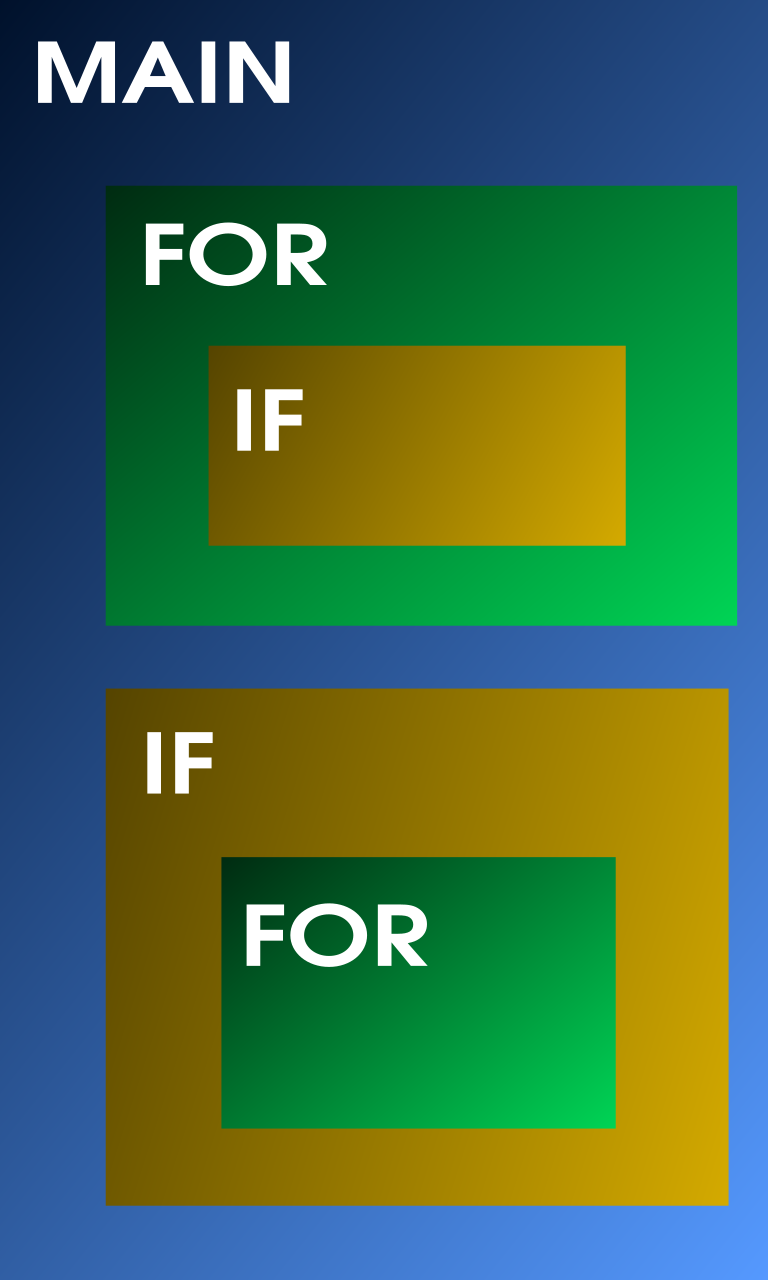
\includegraphics[width=5cm, keepaspectratio]{indentation/Indendacao_1.png}
    \caption{Abstração de blocos de código indentados.}
    \label{fig:indentado}
\end{figure}

\par\tab Porém, caso o mesmo código não esteja indentado, obter-se-á a seguinte impressão:

\begin{figure}[H]
    \centering
    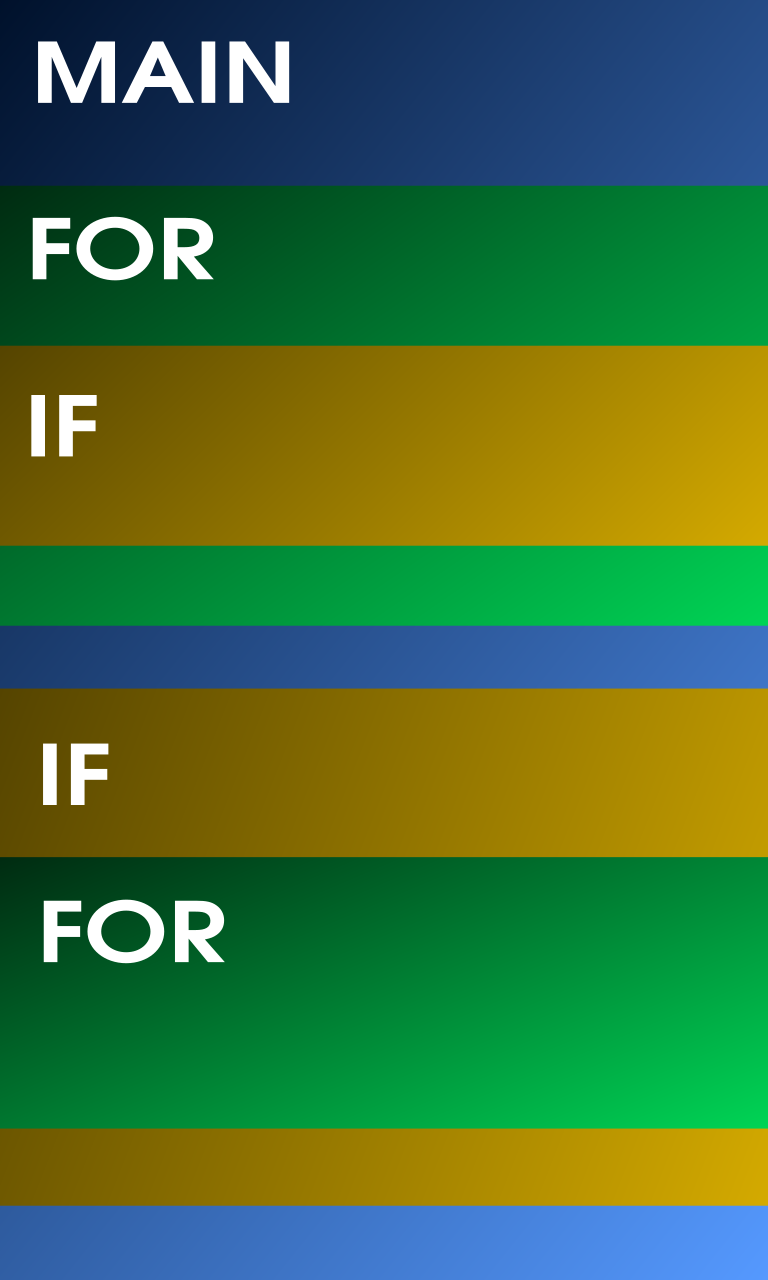
\includegraphics[width=5cm, keepaspectratio]{indentation/Indendacao_2.png}
    \caption{Abstração de blocos de código não indentados.}
    \label{fig:nao_indentado}
\end{figure}

\par\tab É possível notar que toda a ideia de "hierarquia" presente no esquema anterior foi perdida, o que dificulta, e muito, a depuração de um código.

\par\tab Portanto, é altamente recomendado que se insira um recuo (normalmente uma tabulação (\textit{tab}) ou quatro caracteres de espaço seguidos (esta última opção é menos usual, por questões de praticidade)) nas seguintes ocasiões:

\begin{enumerate}
    \item Código contido entre novas chaves abertas: Neste caso, a quantidade de tabulações, por exemplo, será diretamente proporcional à quantidade de chaves abertas em um código (imagine um \textit{if} dentro de um \textit{for}, que por sua vez encontra-se dentro da função \textit{main}. Note que como a função \textit{main}, por si só já abre uma chave, portanto, tanto a instução \textit{for} quanto todo o bloco de código contido nela receberá uma tabulação com relação ao \textit{main}. Quanto ao conteúdo que encontra-se dentro do \textit{for}, também deve receber mais um recuo (inclusive o \textit{if}), uma vez que há duas chaves abertas e, portanto, terão dois recuos com relação ao \textit{main}. Por fim, note que a instrução \textit{if} também abriu novas chaves, portanto, todo o conteúdo contido dentro desta instrução deverá receber mais um recuo (perceba que já são três com relação ao \textit{main}, exatamente a quantidade de chaves atualmente abertas)).
    \item Bloco de código pertencente à um condicional ou à algum laço de repetição: Mesmo que não sejam adicionadas chaves é de bom tom que se dê uma tabulação no bloco afetado pelo condicional ou laço de repetição.
    \item Instruções não acabadas: Existem linhas de código que, por vezes, são muito compridas e ficam visualmente desagradáveis se deixadas na mesma linha (como quando é necessário incluir \textit{strings} grandes, que não cabem em uma linha só). Neste caso, a cada quebra de linha, insere-se uma tabulação (apenas um recuo com relação à linha onde a instrução foi iniciada é suficiente).
\end{enumerate}

\par\tab A seguir um exemplo de código corretamente indentado e outro mal indentado (e com trechos sem indentação). Observe que o primeiro é mais fácil de compreender e mais agradável de se observar (mais elegante):

\hspace{0.25cm}
\begin{lstlisting}
    #include <stdio.h>
    
    int main(int argc, char *argv[]){
        int my_array[10], i;
        
        for (i = 0; i < 10; ++i){
            scanf("%d", my_array + i);
        }
        
        for (i = 0; i < 10; ++i){
            printf("%d ", my_array[i]);
        }
        
        return 0;
    }
\end{lstlisting}

\hspace{0.25cm}
\begin{lstlisting}
    #include <stdio.h>
    
    int main(int argc, char *argv[]){
    int my_array[10], i;
        
        for (i = 0; i < 10; ++i){
            scanf("%d", my_array + i);
    }
        
    for (i = 0; i < 10; ++i){
    printf("%d ", my_array[i]);
    }
        
                return 0;
    }
\end{lstlisting}

\hspace{0.25cm}
\begin{tcolorbox}[colback=yellow!5!white,colframe=yellow!75!black,title=Atenção!]
  \par\tab Não inclua tabulações desnecessárias (aleatoriamente) no código, pois, bem como a falta de tabulação deixa o código deselegante, o excesso também o deixa.
  \par\tab Também tome cuidado para com a tabulação dos fechamentos de chave, pois, se elas não estiverem emparelhadas com sua respectiva chave de abertura, poderá dificultar (e confundir) a interpretação do código. Para mais detalhes, consulte exemplos nos slides de aula de Vetores e Funções do Prof. Dr. Paulo Henrique Pisani \cite{presentation:pe_vet_func}.
\end{tcolorbox}

\subsection{Espaçamento entre linhas}

\par\tab O espaçamento entre linhas também é de extrema importância para deixar o código mais elegante. Ele facilita perceber a separação de blocos/trechos de código que executam partes específicas em uma função.

\par\tab Observe que no trecho de código a seguir, a indentação não é suficiente para deixar o código elegante:

\hspace{0.25cm}
\begin{lstlisting}
    #include <stdio.h>
    int main(int argc, char *argv[]){
        int my_array[10], i;
        for (i = 0; i < 10; ++i){
            scanf("%d", my_array + i);
        }
        for (i = 0; i < 10; ++i){
            printf("%d ", my_array[i]);
        }
        return 0;
    }
\end{lstlisting}

\par\tab Ao inserir o espaçamento adequado, obtemos um código mais elegante (note que eles são idênticos):

\hspace{0.25cm}
\begin{lstlisting}
    #include <stdio.h>
    
    int main(int argc, char *argv[]){
        int my_array[10], i;
        
        for (i = 0; i < 10; ++i){
            scanf("%d", my_array + i);
        }
        
        for (i = 0; i < 10; ++i){
            printf("%d ", my_array[i]);
        }
        
        return 0;
    }
\end{lstlisting}

\par\tab É importante lembrar que deve-se utilizar o espaçamento de forma consciente, evitando excessos e, como consequência, um código mais poluído que o anterior:

\hspace{0.25cm}
\begin{lstlisting}
    #include <stdio.h>
    
    int main(int argc, char *argv[]){
        int my_array[10], i;
        
        
        for (i = 0; i < 10; ++i){
            scanf("%d", my_array + i);
        }
        
        
        
        
        for (i = 0; i < 10; ++i){
            printf("%d ", my_array[i]);
        }
        
        
        return 0;
    }
\end{lstlisting}

\subsection{Declaração de constantes}

\par\tab Ao declarar constantes (incluindo alguns tipos de enumerador), tem-se o costume de declará-las com o identificador em caixa alta, assim, fica mais fácil identificar quais são os valores mais importantes/utilizados em um programa.

\par\tab A seguir, alguns exemplos de quando utilizar caixa alta:

\hspace{0.25cm}
\begin{lstlisting}
    #define PI 3.14
    #difine VEL_LUZ 299792458
    
    const int MEU_INTEIRO_CONSTANTE = 904;
    
    enum Meses {
        JANEIRO = 1,
        FEVEREIRO = 2,
        //...
        NOVEMBRO = 11,
        DEZEMBRO = 12
    };
\end{lstlisting}

\subsection{Análise de avisos e erros de compilação}

\par\tab Ao desenvolver programas/aplicações é necessário que se saiba encontrar erros que possam ter sido cometidos durante a elaboração do algoritmo. Para isso, pode-se contar com uma ajuda do compilador, que dará dicas e informações a respeito de erros que possam ter passado despercebido durante o processo de desenvolvimento.

\hspace{0.25cm}
\begin{tcolorbox}[colback=blue!5!white,colframe=blue!75!black,title=Dica!]
  \par\tab Embora nos exemplos citados nesta seção sejam dependentes do compilador \textbf{gnu-gcc} (nativamente disponível em praticamente qualquer distribuição Linux ou através do MinGW no Windows), outros compiladores (como os contidos no Dev-C++, VisualStudio, C++ Builder, entre outros) também emitem os mesmos alertas, talvez exibindo mensagens um pouco diferentes, mas que apontam para os mesmos problemas.
  \par\tab Caso seja utilizada uma IDE para a edição do código, como alguma das citadas anteriormente, normalmente ao tentar compilar, as linhas que apresentarem problemas ficarão realçadas (algumas vezes com caixas de ajuda contendo a mensagem de erro), facilitando ainda mais a depuração.
\end{tcolorbox}

\par\tab Como citado anteriormente, além dos erros de compilação, o GCC também pode emitir avisos a respeito de erros no código, mas para isso é necessário incluir a bandeira (\textit{flag}) "\textbf{-Wall}" no comando de compilação, assim ele emitirá todos os avisos possíveis a respeito de prováveis erros. O exemplo a seguir é um comando de compilação para o algoritmo contido no arquivo "teste.c" que gerará um arquivo de saída chamado "a.out" e emitirá todos os avisos possíveis:

\hspace{0.25cm}
\begin{tcolorbox}[colback=black!5!white,colframe=black!75!white,title=Console: usuario@fedora:\~/Exemplos]
    \par gcc teste.c -Wall
\end{tcolorbox}

\par\tab Agora que foi visto como indicar ao compilador para sinalizar mais erros no código, serão apresentados exemplos a seguir, de códigos problemáticos mais recorrentes e suas respectivas mensagens de erros e avisos.

\par\tab\textbf{Falta de ponto e vírgula}
\par\tab Note que há um ponto e vírgula faltando na linha 4 do código fonte.

\hspace{0.25cm}
\begin{lstlisting}
    #include <stdio.h>
    
    int main(int argc, char *argv[]){
        int my_array[10], i
        
        for (i = 0; i < 10; ++i){
            scanf("%d", my_array + i);
        }
        
        for (i = 0; i < 10; ++i){
            printf("%d ", my_array[i]);
        }
        
        return 0;
    }
\end{lstlisting}

\par\tab Saída do console:

\hspace{0.25cm}
\begin{tcolorbox}[colback=black!5!white,colframe=black!75!white,title=Console: usuario@fedora:\~/Exemplos]
    \begin{verbatim}
[usuario@fedora Exemplos]$ gcc teste.c -Wall
teste.c: In function ‘main’:
teste.c:6:9: error: expected ‘=’, ‘,’, ‘;’, ‘asm’ or
‘__attribute__’ before ‘for’
         for (i = 0; i < 10; ++i){
         ^~~
teste.c:6:21: error: ‘i’ undeclared (first use in this function)
         for (i = 0; i < 10; ++i){
                     ^
teste.c:6:21: note: each undeclared identifier is reported only
once for each function it appears in
teste.c:6:32: error: expected ‘;’ before ‘)’ token
         for (i = 0; i < 10; ++i){
                                ^
                                ;
teste.c:6:32: error: expected statement before ‘)’ token
    \end{verbatim}
\end{tcolorbox}

\par\tab Perceba que erros relacionados à ponto e vírgula aparecem como se fosse erro na instrução posterior (neste caso, no \textit{for}). Portanto, nestes casos, sugere-se identificar todas as dicas que a mensagem possui. Logo na primeira informação que temos, o compilador informa que está faltando alguma coisa antes da expressão \textit{for} (chega a sugerir, inclusive, que está faltando um ';'). Já a segunda mensagem informa que o 'i' não foi declarado, mais uma dica importante, já que ao analisar a linha em que o 'i' foi declarado, notar-se-á que falta o ';'.

\hspace{0.25cm}
\begin{tcolorbox}[colback=yellow!5!white,colframe=yellow!75!black,title=Atenção!]
  \par\tab A mensagem de erro onde falta ';' varia dependendo da instrução seguinte.
\end{tcolorbox}

\hspace{2cm}
\par\tab\textbf{Falta de fechamento de chaves}

\par\tab Note que há uma chave faltando na linha 8 do código fonte.

\hspace{0.25cm}
\begin{lstlisting}
    #include <stdio.h>
    
    int main(int argc, char *argv[]){
        int my_array[10], i;
        
        for (i = 0; i < 10; ++i){
            scanf("%d", my_array + i);
        
        for (i = 0; i < 10; ++i){
            printf("%d ", my_array[i]);
        }
        
        return 0;
    }
\end{lstlisting}

\par\tab Saída do console:

\hspace{0.25cm}
\begin{tcolorbox}[colback=black!5!white,colframe=black!75!white,title=Console: usuario@fedora:\~/Exemplos]
    \begin{verbatim}
[usuario@fedora Exemplos]$ gcc teste.c -Wall
teste.c: In function ‘main’:
teste.c:14:5: error: expected declaration or statement at end of
input
     }
     ^
    \end{verbatim}
\end{tcolorbox}

\par\tab Note que neste caso, o compilador só informa que está faltando o fechamento de uma chave, sem especificar com precisão onde esta chave deve ser fechada. Neste caso, é necessário analisar a função inteira para checar onde está faltando.

\hspace{0.25cm}
\begin{tcolorbox}[colback=yellow!5!white,colframe=yellow!75!black,title=Atenção!]
  \par\tab Note que se o código não estiver indentado, será muito mais difícil identificar onde está faltando o fechamento da chave.
\end{tcolorbox}

\hspace{2cm}
\par\tab\textbf{Parâmetro de função incorreto}

\par\tab No exemplo a seguir, as funções \textit{scanf} e \textit{soma} devem receber como segundo e terceiro parâmetro dois ponteiros para inteiro e dois valores para inteiro respectivamente, porém, outros tipos de valores são fornecidos.

\hspace{0.25cm}
\begin{lstlisting}
    #include <stdio.h>
    #include <stdlib.h>
    
    int soma(int a, int b);
    
    int main(){
            char a;
            int b;
    
            scanf("%d %d", &a, &b);
            printf("%d\n", soma(a, b));
    
            return EXIT_SUCCESS;
    }
    
    int soma(int a, int b){
            return a + b;
    }
\end{lstlisting}

\par\tab Saída do console:

\hspace{0.25cm}
\begin{tcolorbox}[colback=black!5!white,colframe=black!75!white,title=Console: usuario@fedora:\~/Exemplos]
    \begin{verbatim}
[usuario@fedora Exemplos]$ gcc teste.c -Wall
teste.c: In function ‘main’:
teste.c:10:10: warning: format ‘%d’ expects argument of type 
‘int *’, but argument 2 has type ‘char *’ [-Wformat=]
  scanf("%d %d", &a, &b);
         ~^      ~~
         %hhd
    \end{verbatim}
\end{tcolorbox}

\par\tab É possível perceber que erros de tipagem de ponteiros são muito mais críticos que de tipagem de dados em si (o C tenta realizar o \textit{casting} implícito sempre que possível entre tipos de dados, já ao trabalhar com ponteiros, a dimensão da variável não pode ser convertida, podendo causar erro de acesso na memória).

\hspace{0.25cm}
\begin{tcolorbox}[colback=yellow!5!white,colframe=yellow!75!black,title=Atenção!]
  \par\tab Note que o compilador não acusou nenhum erro, apenas deu avisos sobre um problema em potencial. Portanto, o programa foi compilado e poderá sofrer vários problemas durante a execução.
\end{tcolorbox}

\hspace{2cm}
\par\tab\textbf{Função sem retorno}

\par\tab Algumas vezes, ao implementar uma função (não procedimento), esquece-se de retornar o resultado, o que torna-a praticamente inútil.

\hspace{0.25cm}
\begin{lstlisting}
    #include <stdio.h>
    #include <stdlib.h>
    
    int soma(int a, int b);
    
    int main(){
            int a, b;
    
            scanf("%d %d", &a, &b);
            printf("%d\n", soma(a, b));
    
            return EXIT_SUCCESS;
    }
    
    int soma(int a, int b){
            int r = a + b;
    }
\end{lstlisting}

\par\tab Saída do console:

\hspace{0.25cm}
\begin{tcolorbox}[colback=black!5!white,colframe=black!75!white,title=Console: usuario@fedora:\~/Exemplos]
    \begin{verbatim}
[usuario@fedora Exemplos]$ gcc teste.c -Wall
teste.c: In function ‘soma’:
teste.c:16:6: warning: unused variable ‘r’ [-Wunused-variable]
  int r = a + b;
      ^
teste.c:17:1: warning: control reaches end of non-void function
[-Wreturn-type]
 }
 ^
    \end{verbatim}
\end{tcolorbox}

\par\tab Neste caso, o compilador identificou dois possíveis problemas:
\begin{enumerate}
    \item \textbf{Variável não usada:} Neste caso, r é uma variável que foi criada, inicializada, mas não foi usada para qualquer coisa depois disso, desperdiçando recursos computacionais. Caso a variável tenha algum valor importante para a função na qual foi criada, então, há um indício de que há algum erro lógico na programação.
    \item \textbf{Função (não procedimento) sem valor de retorno:} Aqui o compilador identificou uma função possivelmente problemática, uma vez que devia retornar um certo valor, mas em sua implementação não há qualquer variável/valor sendo retornada(o).
\end{enumerate}

\subsection{Erros lógicos no algoritmo}

\par\tab Encontrar erros lógicos no algoritmo é muito mais complicado que encontrar erros semânticos, pois, normalmente o erro acontece durante a execução da aplicação e não dá o menor sinal de onde pode ter ocorrido. A seguir serão analisados dois exemplos de erros que passarão despercebidos pelo compilador, mas que farão com que o programa seja encerrado (ou que se comporte de forma inesperada).

\hspace{2cm}
\par\tab\textbf{Variável não inicializada}

\par\tab A seguir, um algoritmo que deveria retornar o maior valor de um vetor.

\hspace{0.25cm}
\begin{lstlisting}
    #include <stdio.h>
    
    int main(int argc, char *argv[]){
        int vetor[10], i;
        
        for (i = 0; i < 10; ++i){
            scanf("%d", vetor + i);
        }
        
        int maior;
        for (i = 0; i < 10; ++i){
            if (vetor[i] > maior){
                maior = vetor[i];
            }
        }
        
        printf("%d\n", maior);
        
        return 0;
    }
\end{lstlisting}

\par\tab Saída do console:

\hspace{0.25cm}
\begin{tcolorbox}[colback=black!5!white,colframe=black!75!white,title=Console: usuario@fedora:\~/Exemplos]
    \begin{verbatim}
[usuario@fedora Exemplos]$ gcc teste.c -Wall
[usuario@fedora Exemplos]$ ./a.out
1 1 1 1 1 1 1 1 1 1
3
    \end{verbatim}
\end{tcolorbox}

\par\tab Note que embora o compilador não tenha identificado nenhum erro em potencial no código, o algoritmo como está possui um erro crítico em relação à função para a qual foi desenvolvido. Ao deixar de inicializar a variável \textbf{maior}, o primeiro valor a ser comparado é um valor qualquer, já contido na memória no momento em que foi alocada, neste caso o \textbf{3}, que sequer estava presente no vetor.

\hspace{0.25cm}
\begin{tcolorbox}[colback=red!5!white,colframe=red!75!black,title=Cuidado!]
  \par\tab Caso a variável não inicializada seja um ponteiro, normalmente o valor "lixo" contido nela é relativamente baixo e não pertencente ao programa atual. Portanto, caso haja a tentativa de acessar a variável contida no endereço apontado, é muito provável que o sistema operacional encerre o processo e apresente a seguinte mensagem de erro: \textbf{\textit{Segmentation fault (imagem do núcleo gravada)}}. Neste caso, normalmente o compilador emite um aviso, devido à gravidade da falha.
\end{tcolorbox}

\hspace{2cm}
\par\tab\textbf{\textit{Casting} implícito}

\par\tab Note que o resultado da divisão de 5 por 2 está sendo armazenado em uma variável inteira, o que acarretará no truncamento do resultado.

\hspace{0.25cm}
\begin{lstlisting}
    #include <stdio.h>
    
    int main(int argc, char *argv[]){
        double a = 5, b = 2;
        int i = a/b;
        
        printf("%d\n", i);
        
        return 0;
    }
\end{lstlisting}

\par\tab Saída do console:

\hspace{0.25cm}
\begin{tcolorbox}[colback=black!5!white,colframe=black!75!white,title=Console: usuario@fedora:\~/Exemplos]
    \begin{verbatim}
[usuario@fedora Exemplos]$ gcc teste.c -Wall
2
    \end{verbatim}
\end{tcolorbox}

\par\tab Perceba o tipo de variável do resultado da operação é \textbf{float}, porém está sendo armazenado em uma variável do tipo \textbf{int}, que além de possuir um intervalo menor de dados, não oferece suporte à variáveis decimais. Logo, o resultado é truncado (ignora casas decimais) e então assinalado à variável \textbf{i}. Portanto, tome cuidado para não realizar \textit{castings} acidentais.

\hspace{2cm}
\par\tab\textbf{Uso de operador de atribuição (=) ao invés de comparação (==) em condicionais e em laços de repetição}

\par\tab Outro erro comum é esquecer-se da diferença entre o operador de atribuição e o de comparação.

\hspace{0.25cm}
\begin{lstlisting}
    #include <stdio.h>
    
    int main(int argc, char *argv[]){
        int i = 2;
        
        if (i = 3){
            printf("O valor de i eh 3\n");
        }
        else {
            printf("O valor de i nao eh 3\n");
        }
        
        return 0;
    }
\end{lstlisting}

\par\tab Saída do console:

\hspace{0.25cm}
\begin{tcolorbox}[colback=black!5!white,colframe=black!75!white,title=Console: usuario@fedora:\~/Exemplos]
    \begin{verbatim}
[usuario@fedora Exemplos]$ gcc teste.c -Wall
[usuario@fedora Exemplos]$ ./a.out
O valor de i eh 3
    \end{verbatim}
\end{tcolorbox}

\par\tab Neste caso, a saída sempre será "O valor de i eh 3", uma vez que o i não está sendo comparado com o 3, mas o número 3 está sendo atribuído à variável i e, em C, o \textit{if} interpreta como verdadeiro caso a atribuição seja realizada com sucesso.

\hspace{2cm}
\par\tab\textbf{Função recursiva sem caso base}

\par\tab A seguir, há a implementação da função de Fibonacci recursiva sem caso base.

\hspace{0.25cm}
\begin{lstlisting}
    #include <stdio.h>
    
    long long int fibonacci(int n);

    int main(){
        printf("%lld\n", fibonacci(100));
    
        return 0;
    }
    
    long long int fibonacci(int n){
        return fibonacci(n-1) + fibonacci(n-2);
    }
\end{lstlisting}

\par\tab Saída do console:

\hspace{0.25cm}
\begin{tcolorbox}[colback=black!5!white,colframe=black!75!white,title=Console: usuario@fedora:\~/Exemplos]
    \begin{verbatim}
[usuario@fedora Exemplos]$ gcc teste.c -Wall
[usuario@fedora Exemplos]$ ./a.out
Segmentation fault (imagem do núcleo gravada)
    \end{verbatim}
\end{tcolorbox}

\par\tab Neste caso, a função \textit{fibonacci} acaba entrando em \textit{loop} infinito, pois, ela sempre recorrerá a ela mesma. Neste caso, o sistema operacional identifica o \textit{loop} e encerra o processo, apresentando a seguinte mensagem de erro: \textbf{\textit{Segmentation fault (imagem do núcleo gravada)}}.

\subsubsection{Depuração de código}

\par\tab Ás vezes, para encontrar o erro causado na execução, ou até mesmo para compreender porque a saída está incorreta, é necessário inserir no código saídas adicionais (\textit{printf}) contendo os valores das variáveis possivelmente problemáticas ou ainda simplesmente para exibir uma série de mensagens "AQUI", facilitando a identificação do ponto onde o programa é interrompido inesperadamente \cite{presentation:debug_c}.

\par\tab A seguir, há um código cujo objetivo é simplesmente efetuar a leitura de um vetor de 10 posições e exibi-lo ao usuário:

\hspace{0.25cm}
\begin{lstlisting}
    #include <stdio.h>
    
    int main(int argc, char *argv[]){
        int vetor[10], i;
        
        for (i = 0; i <= 10; ++i){
            scanf("%d", vetor + i);
        }
        
        for (i = 0; i < 10; ++i){
            printf("%d ", v[i]);
        }
        printf("\n");
        
        return 0;
    }
\end{lstlisting}

\par\tab A saída do console, porém, retornou um erro (note que ele pede o 11 caractere)!

\hspace{0.25cm}
\begin{tcolorbox}[colback=black!5!white,colframe=black!75!white,title=Console: usuario@fedora:\~/Exemplos]
    \begin{verbatim}
[usuario@fedora Exemplos]$ gcc teste.c -Wall
[usuario@fedora Exemplos]$ ./a.out
1 1 1 1 1 1 1 1 1 1 1
Segmentation fault (imagem do núcleo gravada)
    \end{verbatim}
\end{tcolorbox}

\par\tab Para descobrir em que trecho do código o problema ocorre, foram inseridas 3 mensagens adicionais:

\hspace{0.25cm}
\begin{lstlisting}
    #include <stdio.h>
    
    int main(int argc, char *argv[]){
        int vetor[10], i;
        
        printf("AQUI 1");
        for (i = 0; i <= 10; ++i){
            scanf("%d", vetor + i);
        }
        printf("AQUI 2");
        
        for (i = 0; i < 10; ++i){
            printf("%d ", v[i]);
        }
        printf("\n");
        printf("AQUI 3");
        
        return 0;
    }
\end{lstlisting}

\par\tab Agora o console exibiu a seguinte saída:

\hspace{0.25cm}
\begin{tcolorbox}[colback=black!5!white,colframe=black!75!white,title=Console: usuario@fedora:\~/Exemplos]
    \begin{verbatim}
[usuario@fedora Exemplos]$ gcc teste.c -Wall
[usuario@fedora Exemplos]$ ./a.out
AQUI 1
1 1 1 1 1 1 1 1 1 1 1
Segmentation fault (imagem do núcleo gravada)
    \end{verbatim}
\end{tcolorbox}

\par\tab Agora, pela ao analisar a saída, fica mais fácil perceber que o problema ocorre no trecho de código que encontra-se entre o \textit{printf("AQUI 1")} e o \textit{printf("AQUI 2")}.

\par\tab Caso ainda não esteja claro onde o problema está, pode-se inserir mais \textit{printf}s, desta vez, dentro do laço de repetição (neste caso, é interessante acompanhar o valor da variável contadora):

\hspace{0.25cm}
\begin{lstlisting}
    #include <stdio.h>
    
    int main(int argc, char *argv[]){
        int vetor[10], i;
        
        printf("AQUI 1");
        for (i = 0; i <= 10; ++i){
            printf("I = %d\n", i);
            scanf("%d", vetor + i);
        }
        printf("AQUI 2");
        
        for (i = 0; i < 10; ++i){
            printf("%d ", v[i]);
        }
        printf("\n");
        printf("AQUI 3");
        
        return 0;
    }
\end{lstlisting}

\hspace{0.25cm}
\begin{tcolorbox}[colback=black!5!white,colframe=black!75!white,title=Console: usuario@fedora:\~/Exemplos]
    \begin{verbatim}
[usuario@fedora Exemplos]$ gcc teste.c -Wall
[usuario@fedora Exemplos]$ ./a.out
AQUI 1
1 1 1 1 1 1 1 1 1 1 1
I = 0
I = 1
I = 2
I = 3
I = 4
I = 5
I = 6
I = 7
I = 8
I = 9
I = 10
Segmentation fault (imagem do núcleo gravada)
    \end{verbatim}
\end{tcolorbox}

\par\tab Agora ficou claro que o problema ocorre na 11ª iteração do laço de repetição.

\par\tab Ao analisar o código novamente, é possível perceber que o \textit{scanf} tenta acessar a posição 10 do vetor, que não existe. Logo, o erro foi encontrado, bastando, agora, corrigir o código (se já tiver certeza que não há nenhum outro erro, já é possível remover os \textit{printf}s adicionais):

\hspace{0.25cm}
\begin{lstlisting}
    #include <stdio.h>
    
    int main(int argc, char *argv[]){
        int vetor[10], i;
        
        for (i = 0; i < 10; ++i){
            scanf("%d", vetor + i);
        }
        
        for (i = 0; i < 10; ++i){
            printf("%d ", v[i]);
        }
        printf("\n");
        
        return 0;
    }
\end{lstlisting}

\par\tab Desta vez, nenhum erro será exibido:

\hspace{0.25cm}
\begin{tcolorbox}[colback=black!5!white,colframe=black!75!white,title=Console: usuario@fedora:\~/Exemplos]
    \begin{verbatim}
[usuario@fedora Exemplos]$ gcc teste.c -Wall
[usuario@fedora Exemplos]$ ./a.out
1 1 1 1 1 1 1 1 1 1 
1 1 1 1 1 1 1 1 1 1 
    \end{verbatim}
\end{tcolorbox}

\hspace{0.25cm}
\begin{tcolorbox}[colback=blue!5!white,colframe=blue!75!black,title=Dica!]
  \par\tab Você também pode dar uma olhada nos algoritmos disponíveis na página do Professor Dr. Paulo Henrique para verificar outros exemplos de códigos depurados \cite{site:debug_c}.
\end{tcolorbox}

\newpage
\section{Resolução de problemas e algoritmos úteis}

\subsection{Palíndromo}

\par\tab A função recursiva definida pelo protótipo \textit{int eh\_palindroma(char *v, int ini, int fim)} deve identificar se a palavra é palíndroma:

\hspace{0.25cm}
\begin{tcolorbox}[colback=violet!5!white,colframe=violet!75!white,title=Capítulos recomendados:]
    \begin{itemize}
        \item Tipos de dados (tipagem de variáveis): Vetores e matrizes: Vetores;
        \item Tipos de dados (tipagem de variáveis): Ponteiros (e suas respectivas subseções);
        \item Tipos de dados (tipagem de variáveis): Fluxo de dados (entrada e saída): (e suas respectivas subseções);
        \item Estruturas de controle e repetição (e suas respectivas subseções);
        \item Funções (e suas respectivas subseções);
    \end{itemize}
\end{tcolorbox}

\hspace{0.25cm}
\begin{lstlisting}
    #include <stdio.h>
    #include <stdlib.h>
    
    int tamanho_string(char *v, int max);
    int eh_palindroma(char *v, int ini, int fim);
    
    int main(int argc, char *argv[]){
    	char string[2048];
    	
        while (scanf("%s", string) != EOF)
    		printf(eh_palindroma(string, 0, tamanho_string(string, 2048) - 1) ?
    			   	"Eh palindroma.\n" : "Nao eh palindroma.\n");
    
        return EXIT_SUCCESS;
    }
    
    int tamanho_string(char *v, int max){
    	int i;
    	for (i = 0; i < max; ++i)
    		if (v[i] == '\0') return i;
    	return max;
    }
    
    int eh_palindroma(char *v, int ini, int fim){
    	if (fim - ini < 2) return 1;
    	if (v[ini] == v[fim]) return eh_palindroma(v, ++ini, --fim);
    	return 0;
    }
\end{lstlisting}

\newpage
\subsection{Brincando com ponteiros}

\par\tab Este algoritmo tem como simples objetivo melhorar a compreensão do funcionamento de variáveis ponteiro.

\hspace{0.25cm}
\begin{tcolorbox}[colback=violet!5!white,colframe=violet!75!white,title=Capítulos recomendados:]
    \begin{itemize}
        \item Tipos de dados (tipagem de variáveis): Ponteiros (e suas respectivas subseções);
        \item Tipos de dados (tipagem de variáveis): Fluxo de dados (entrada e saída): (e suas respectivas subseções);
    \end{itemize}
\end{tcolorbox}

\hspace{0.25cm}
\begin{lstlisting}
    #include <stdio.h>
    #include <stdlib.h>
    
    int main(int argc, char *argv[]){
    	int var = 7;
    	printf("%d\n", var); 		// imprime 7
    	printf("%p\n", &var); 		// imprime o endereco de var
    
    	int *end_var;
    	end_var = &var; 			// end_var = endereco de var
    
    	printf("%p\n", end_var); 	// imprime o endereco de var em hexadecimal
    	printf("%lld\n", end_var); 	// imprime o endereco de var em decimal
    
    	//Essas duas linhas sao iguais
    	printf("%d\n", *end_var); 	// imprime 7
    	printf("%d\n", *(&var));  	// imprime 7
    	//-----------------------------------------------------------------
    	*end_var = 9;
    
    	printf("%p\n", end_var);
    	printf("%d\n", *end_var); 	// imprime 9
    	printf("%d\n", var); 		// imprime 9
    	
    	return EXIT_SUCCESS;
    }
\end{lstlisting}

\newpage

\subsection{Bubble Sort}

\hspace{0.25cm}
\begin{tcolorbox}[colback=violet!5!white,colframe=violet!75!white,title=Capítulos recomendados:]
    \begin{itemize}
        \item Tipos de dados (tipagem de variáveis): Tipos primitivos: Inteiro;
        \item Tipos de dados (tipagem de variáveis): Vetores e matrizes: Vetores;
        \item Tipos de dados (tipagem de variáveis): Ponteiros (e suas respectivas subseções);
        \item Tipos de dados (tipagem de variáveis): Fluxo de dados (entrada e saída): (e suas respectivas subseções);
        \item Estruturas de controle e repetição (e suas respectivas subseções);
    \end{itemize}
\end{tcolorbox}

\hspace{0.25cm}
\begin{lstlisting}
    #include <stdio.h>
    #include <stdlib.h>
        
    int main(int argc, char *argv[]){
        int n, i, j;
        scanf("%d", &n);
            
        int *v = (int*)malloc(n * sizeof(int));
        for (i = 0; i < n; ++i)
                scanf("%d", v+i);
    
        for (i = 0; i < n; ++i)
    		for (j = 0; j < n - i - 1; ++j)
                if (v[j+1] < v[j]){
                    int temp = v[j];
                    v[j] = v[j+1];
                    v[j+1] = temp;
                }
        
        printf("Vetor ordenado:\n");
        for (i = 0; i < n; ++i)
            printf("%d%c", v[i], i == n-1 ? '\n' : ' ');
            
        free(v);
        
        return EXIT_SUCCESS;
    }
\end{lstlisting}

\newpage
\subsection{Insertion Sort}

\hspace{0.25cm}
\begin{tcolorbox}[colback=violet!5!white,colframe=violet!75!white,title=Capítulos recomendados:]
    \begin{itemize}
        \item Tipos de dados (tipagem de variáveis): Tipos primitivos: Inteiro;
        \item Tipos de dados (tipagem de variáveis): Vetores e matrizes: Vetores;
        \item Tipos de dados (tipagem de variáveis): Ponteiros (e suas respectivas subseções);
        \item Tipos de dados (tipagem de variáveis): Fluxo de dados (entrada e saída): (e suas respectivas subseções);
        \item Estruturas de controle e repetição (e suas respectivas subseções);
    \end{itemize}
\end{tcolorbox}

\hspace{0.25cm}
\begin{lstlisting}
    #include <stdio.h>
    #include <stdlib.h>
        
    int main(int argc, char *argv[]){
        int n, i, j;
        scanf("%d", &n);
            
        int *v = (int*)malloc(n * sizeof(int));
        for (i = 0; i < n; ++i)
                scanf("%d", v+i);
    
        for (i = 1; i < n; ++i){
            int pos = i, valor = v[i];
    		for (j = i - 1; j > -1 && v[j] > valor; --j){
    		    v[j+1] = v[j];
    		    pos--;
    		}
    		v[pos] = valor;
        }
        
        printf("Vetor ordenado:\n");
        for (i = 0; i < n; ++i)
            printf("%d%c", v[i], i == n-1 ? '\n' : ' ');
        free(v);
        
        return EXIT_SUCCESS;
    }
\end{lstlisting}

\newpage
\subsection{Selection Sort}

\hspace{0.25cm}
\begin{tcolorbox}[colback=violet!5!white,colframe=violet!75!white,title=Capítulos recomendados:]
    \begin{itemize}
        \item Tipos de dados (tipagem de variáveis): Tipos primitivos: Inteiro;
        \item Tipos de dados (tipagem de variáveis): Vetores e matrizes: Vetores;
        \item Tipos de dados (tipagem de variáveis): Ponteiros (e suas respectivas subseções);
        \item Tipos de dados (tipagem de variáveis): Fluxo de dados (entrada e saída): (e suas respectivas subseções);
        \item Estruturas de controle e repetição (e suas respectivas subseções);
    \end{itemize}
\end{tcolorbox}

\hspace{0.25cm}
\begin{lstlisting}
    #include <stdio.h>
    #include <stdlib.h>
        
    int main(int argc, char *argv[]){
        int n, i, j;
        scanf("%d", &n);
            
        int *v = (int*)malloc(n * sizeof(int));
        for (i = 0; i < n; ++i)
    		scanf("%d", v+i);
    
        for (i = 0; i < n - 1; ++i){
    		int menor = i;
    		for (j = i + 1; j < n; ++j)
    			if (v[menor] > v[j])
    				menor = j;
    		
    		if (i != menor){
    			int temp = v[menor];
    			v[menor] = v[i];
    			v[i] = temp;
    		}
    	}
    	
        printf("Vetor ordenado:\n");
        for (i = 0; i < n; ++i)
            printf("%d%c", v[i], i == n-1 ? '\n' : ' ');
            
    	free(v);
    	
        return EXIT_SUCCESS;
    }
\end{lstlisting}

\newpage
\subsection{Busca Binária}

\hspace{0.25cm}
\begin{tcolorbox}[colback=violet!5!white,colframe=violet!75!white,title=Capítulos recomendados:]
    \begin{itemize}
        \item Tipos de dados (tipagem de variáveis): Vetores e matrizes: Vetores;
        \item Tipos de dados (tipagem de variáveis): Fluxo de dados (entrada e saída): (e suas respectivas subseções);
        \item Estruturas de controle e repetição (e suas respectivas subseções);
        \item Funções (e suas respectivas subseções);
    \end{itemize}
\end{tcolorbox}

\hspace{0.25cm}
\begin{lstlisting}
    #include <stdio.h>
    #include <stdlib.h>
    
    int busca_bin(int v[], int tam, int k);
    
    int main(int argc, char *argv[]){
        int n, i;
        scanf("%d", &n);
        
    	printf("Digite os valores do vetor ORDENADO:\n");
        int *v = (int*)malloc(n * sizeof(int));
        for (i = 0; i < n; ++i)
                scanf("%d", v+i);
        
    	printf("Digite um numero a ser buscado no vetor: ");
        while (scanf("%d", &i) != EOF){
    		int k = busca_bin(v, n, i);
    		if (k != -1) printf("O valor encontra-se na posicao %d do vetor\n", k);
    		else printf("Este valor nao esta no vetor\n");
    		printf("Digite um numero a ser buscado no vetor: ");
    	}
    	printf("\n");
    	
    	free(v);
            
        return EXIT_SUCCESS;
    }
    
    int busca_bin(int v[], int tam, int k){
    	int ini = 0, fim = tam - 1;
    	
    	while(ini <= fim){
    		int meio = (ini + fim)/ 2;
    		
    		if (v[meio] == k) return meio;
    		else if (v[meio] > k) fim = meio - 1;
    		else ini = meio + 1;
    	}
    	return -1;
    }
\end{lstlisting}

\newpage
\subsection{Busca Binária - Recursiva}

\hspace{0.25cm}
\begin{tcolorbox}[colback=violet!5!white,colframe=violet!75!white,title=Capítulos recomendados:]
    \begin{itemize}
        \item Tipos de dados (tipagem de variáveis): Vetores e matrizes: Vetores;
        \item Tipos de dados (tipagem de variáveis): Fluxo de dados (entrada e saída): (e suas respectivas subseções);
        \item Estruturas de controle e repetição (e suas respectivas subseções);
        \item Funções (e suas respectivas subseções);
    \end{itemize}
\end{tcolorbox}

\hspace{0.25cm}
\begin{lstlisting}
    #include <stdio.h>
    #include <stdlib.h>
    
    int busca_bin(int n, int v[], int ini, int fim);
    
    int main(int argc, char *argv[]){
        int n, i;
        scanf("%d", &n);
        
    	printf("Digite os valores do vetor ORDENADO:\n");
        int *v = (int*)malloc(n * sizeof(int));
        for (i = 0; i < n; ++i)
                scanf("%d", v+i);
        
    	printf("Digite um numero a ser buscado no vetor: ");
        while (scanf("%d", &i) != EOF){
    		int k = busca_bin(i, v, 0, n-1);
    		if (k != -1) printf("O valor encontra-se na posicao %d do vetor\n", k);
    		else printf("Este valor nao esta no vetor\n");
    		printf("Digite um numero a ser buscado no vetor: ");
    	}
    	printf("\n");
        
        free(v);
        
        return EXIT_SUCCESS;
    }
    
    int busca_bin(int n, int v[], int ini, int fim){
    	if (ini > fim) return -1;
    	int meio = (ini + fim)/ 2;
    	
    	if (v[meio] == n) return meio;
    	
    	if (v[meio] > n) return busca_bin(n, v, ini, meio - 1);
    	else return busca_bin(n, v, meio + 1, fim);
    }
\end{lstlisting}

\newpage
\subsection{Fibonacci}

\hspace{0.25cm}
\begin{tcolorbox}[colback=violet!5!white,colframe=violet!75!white,title=Capítulos recomendados:]
    \begin{itemize}
        \item Tipos de dados (tipagem de variáveis): Tipos primitivos: Inteiro;
        \item Tipos de dados (tipagem de variáveis): Vetores e matrizes: Vetores;
        \item Tipos de dados (tipagem de variáveis): Fluxo de dados (entrada e saída): (e suas respectivas subseções);
        \item Estruturas de controle e repetição (e suas respectivas subseções);
    \end{itemize}
\end{tcolorbox}

\hspace{0.25cm}
\begin{lstlisting}
    #include <stdio.h>
    #include <stdlib.h>
        
    int main(int argc, char *argv[]){
    	int i;
        long int fibonacci[90];
           
        fibonacci[0] = 0;
    	fibonacci[1] = 1;
        for (i = 2; i < 90; ++i)
            fibonacci[i] = fibonacci[i - 1] + fibonacci[i - 2];
            
        while (scanf("%d", &i) != EOF)
            if (i < 90 && i > -1) printf("F(%d) = %ld\n", i,fibonacci[i]);
            else printf("Numero fora do intervalo [0 : 89]\n");
            
        return EXIT_SUCCESS;
    }
\end{lstlisting}

\newpage
\subsection{Fibonacci - Recursivo}

\hspace{0.25cm}
\begin{tcolorbox}[colback=violet!5!white,colframe=violet!75!white,title=Capítulos recomendados:]
    \begin{itemize}
        \item Tipos de dados (tipagem de variáveis): Tipos primitivos: Inteiro;
        \item Tipos de dados (tipagem de variáveis): Fluxo de dados (entrada e saída): (e suas respectivas subseções);
        \item Funções (e suas respectivas subseções);
    \end{itemize}
\end{tcolorbox}

\hspace{0.25cm}
\begin{lstlisting}
    #include <stdio.h>
    #include <stdlib.h>
    
    long int fibonacci(int n);
    
    int main(int argc, char *argv[]){
    	int i;
    
        while (scanf("%d", &i) != EOF)
            if (i > -1) printf("F(%d) = %ld\n", i,fibonacci(i));
            else printf("Numero fora do intervalo [x >= 0]\n");
            
        return EXIT_SUCCESS;
    }
    
    long int fibonacci(int n){
    	if (!n) return 0;
    	if (n == 1) return 1;
    	if (n < 0) return -1;
    	
    	return fibonacci(n-1) + fibonacci(n-2);
    }
\end{lstlisting}

\newpage
\subsection{Fibonacci - Programação Dinâmica (Bottom-Up)}

\hspace{0.25cm}
\begin{tcolorbox}[colback=violet!5!white,colframe=violet!75!white,title=Capítulos recomendados:]
    \begin{itemize}
        \item Tipos de dados (tipagem de variáveis): Tipos primitivos: Inteiro;
        \item Tipos de dados (tipagem de variáveis): Vetores e matrizes: Vetores;
        \item Tipos de dados (tipagem de variáveis): Fluxo de dados (entrada e saída): (e suas respectivas subseções);
        \item Estruturas de controle e repetição (e suas respectivas subseções);
        \item Funções (e suas respectivas subseções);
    \end{itemize}
\end{tcolorbox}

\hspace{0.25cm}
\begin{lstlisting}
    #include <stdio.h>
    #include <stdlib.h>
    
    long int fibonacci(int n, long int v[], int tam);
    
    int main(int argc, char *argv[]){
    	int i;
        long int fib[90];
    
        fib[0] = 0;
    	fib[1] = 1;
        for (i = 2; i < 90; ++i)
            fib[i] = -1;
            
        while (scanf("%d", &i) != EOF)
            if (i < 90 && i > -1) printf("F(%d) = %ld\n", i, fibonacci(i, fib, 90));
            else printf("Numero fora do intervalo [0 : 89]\n");
            
        return EXIT_SUCCESS;
    }
    
    long int fibonacci(int n, long int v[], int tam){
    	if (!n) return 0;
    	if (n == 1) return 1;
    	if (n >= tam || n < 0) return -1;
    	
    	if (v[n] < 0)
    		v[n] = fibonacci(n-1, v, tam) + fibonacci(n-2, v, tam);
    	return v[n];
    }
\end{lstlisting}

\newpage
\subsection{[Estrutura de dados] Pilha (Dinâmica)}

\hspace{0.25cm}
\begin{tcolorbox}[colback=violet!5!white,colframe=violet!75!white,title=Capítulos recomendados:]
    \begin{itemize}
        \item Tipos de dados (tipagem de variáveis): Tipos abstratos de dados;
        \item Tipos de dados (tipagem de variáveis): Fluxo de dados (entrada e saída): (e suas respectivas subseções);
        \item Tipos de dados (tipagem de variáveis): Ponteiros (e suas respectivas subseções);
        \item Estruturas de controle e repetição (e suas respectivas subseções);
        \item Funções (e suas respectivas subseções);
        \item \textbf{Linguagem C: typedef \cite{site:typedef}.}
    \end{itemize}
\end{tcolorbox}

\hspace{0.25cm}
\begin{lstlisting}
    #include <stdio.h>
    #include <stdlib.h>
    #include <string.h>
    
    //Se precisar de uma pilha de outro tipo, basta substituir o "int" pelo tipo desejado (cuidado com o scanf e printf)
    typedef int datatype;
    
    typedef struct tItem{
    	datatype data;
    	struct tItem *next;
    } Item;
    
    typedef struct tStack{
    	Item *top;
    	int size;
    } Stack;
    
    Stack* createStack();
    
    Item* pop(Stack *s);
    Item* createItem(datatype value);
    int push(Stack *s, datatype value);
    int stackSize(Stack *s);
    datatype topValue(Stack *s);
    
    int main(int argc, char *argv[]){
    	Stack *myStack = createStack();
    	if (!myStack){
    		printf("Nao foi possivel criar a pilha.\n");
    		return EXIT_FAILURE;
    	}
    	char op[2] = "o";
    	int valor;
    	do{
    		if (!strcmp(op, "M")) printf("%d\n", topValue(myStack));
    		else if (!strcmp(op ,"T")) printf("%d\n", stackSize(myStack));
    		else if (!strcmp(op ,"P")) {
    			Item *i = pop(myStack);
    			printf("%d\n", i->data);
    			free(i);
    		}
    		else if (!strcmp(op ,"E")){
    			scanf("%d", &valor);
    			push(myStack, valor);
    		}
    		printf("Selecione uma opcao:\n"
    			   "M - Mostra o valor do topo.\n"
    			   "P - Mostra o valor do topo e desempilha ele.\n"
    			   "E <valor> - Empilha o valor desejado.\n"
    			   "T - Mostra o tamanho da pilha.\n");
    		
    	} while(scanf("%s", op) != EOF);
    	
    	free(myStack);
    	
    	return EXIT_SUCCESS;
    }
    
    Stack* createStack(){
    	Stack *newStack = (Stack*)malloc(sizeof(Stack));
    	if (!newStack) return NULL;
    	
    	newStack->top = NULL;
    	newStack->size = 0;
    	
    	return newStack;
    }
    
    Item* pop(Stack *s){
    	if (!s->top) return NULL;
    	
    	Item *oldTop = s->top;
    	s->top = oldTop->next;
    	s->size--;
    	
    	return oldTop;
    }
    
    Item* createItem(datatype value){
    	Item *newItem = (Item*)malloc(sizeof(Item));
    	if (!newItem) return NULL;
    	
    	newItem->next = NULL;
    	newItem->data = value;
    	
    	return newItem;
    }
    
    int push(Stack *s, datatype value){
    	Item *newItem = createItem(value);
    	if (!newItem) return 0;
    	
    	newItem->next = s->top;
    	s->top = newItem;
    	s->size++;
    	
    	return 1;
    }
    
    int stackSize(Stack *s){
    	return s->size;
    }
    
    datatype topValue(Stack *s){
    	if (s->size) return s->top->data;
    	return 0;
    }
\end{lstlisting}

\newpage
\subsection{[Estrutura de dados] Fila (Dinâmica)}

\hspace{0.25cm}
\begin{tcolorbox}[colback=violet!5!white,colframe=violet!75!white,title=Capítulos recomendados:]
    \begin{itemize}
        \item Tipos de dados (tipagem de variáveis): Tipos abstratos de dados;
        \item Tipos de dados (tipagem de variáveis): Fluxo de dados (entrada e saída): (e suas respectivas subseções);
        \item Tipos de dados (tipagem de variáveis): Ponteiros (e suas respectivas subseções);
        \item Estruturas de controle e repetição (e suas respectivas subseções);
        \item Funções (e suas respectivas subseções);
        \item \textbf{Linguagem C: typedef \cite{site:typedef}.}
    \end{itemize}
\end{tcolorbox}

\hspace{0.25cm}
\begin{lstlisting}
    #include <stdio.h>
    #include <stdlib.h>
    #include <string.h>
    
    //Se precisar de uma fila de outro tipo, basta substituir o "int" pelo tipo desejado (cuidado com o scanf e printf)
    typedef int datatype;
    
    typedef struct tItem{
    	datatype data;
    	struct tItem *next;
    } Item;
    
    typedef struct tQueue{
    	Item *first;
    	int size;
    } Queue;
    
    Queue* createQueue();
    
    Item* removeItem(Queue *s);
    Item* createItem(datatype value);
    int insert(Queue *s, datatype value);
    int queueSize(Queue *s);
    datatype firstValue(Queue *s);
    
    int main(int argc, char *argv[]){
    	Queue *myQueue = createQueue();
    	if (!myQueue){
    		printf("Nao foi possivel criar a fila.\n");
    		return EXIT_FAILURE;
    	}
    	char op[2] = "o";
    	int valor;
    	do{
    		if (!strcmp(op, "M")) printf("%d\n", firstValue(myQueue));
    		else if (!strcmp(op ,"T")) printf("%d\n", queueSize(myQueue));
    		else if (!strcmp(op ,"R")) {
    			Item *i = removeItem(myQueue);
    			printf("%d\n", i->data);
    			free(i);
    		}
    		else if (!strcmp(op ,"I")){
    			scanf("%d", &valor);
    			insert(myQueue, valor);
    		}
    		printf("Selecione uma opcao:\n"
    			   "M - Mostra o primeiro valor.\n"
    			   "R - Mostra o primeiro valor e desenfila ele.\n"
    			   "I <valor> - Enfila o valor desejado.\n"
    			   "T - Mostra o tamanho da fila.\n");
    		
    	} while(scanf("%s", op) != EOF);
    	
    	free(myQueue);
    	
    	return EXIT_SUCCESS;
    }
    
    Queue* createQueue(){
    	Queue *newQueue = (Queue*)malloc(sizeof(Queue));
    	if (!newQueue) return NULL;
    	
    	newQueue->first = NULL;
    	newQueue->size = 0;
    	
    	return newQueue;
    }
    
    Item* removeItem(Queue *s){
    	if (!s->first) return NULL;
    	
    	Item *oldFirst = s->first;
    	s->first = oldFirst->next;
    	s->size--;
    	
    	return oldFirst;
    }
    
    Item* createItem(datatype value){
    	Item *newItem = (Item*)malloc(sizeof(Item));
    	if (!newItem) return NULL;
    	
    	newItem->next = NULL;
    	newItem->data = value;
    	
    	return newItem;
    }
    
    int insert(Queue *s, datatype value){
    	Item *newItem = createItem(value);
    	if (!newItem) return 0;
    	
    	if (!s->first)
    		s->first = newItem;
    	else {
    		Item *lastItem = NULL, *currentItem = s->first;
    		while(currentItem){
    			lastItem = currentItem;
    			currentItem = currentItem->next;
    		}
    		lastItem->next = newItem;
    	}
    	s->size++;
    	
    	return 1;
    }
    
    int queueSize(Queue *s){
    	return s->size;
    }
    
    datatype firstValue(Queue *s){
    	if (s->size) return s->first->data;
    	return 0;
    }
\end{lstlisting}

\newpage
\subsection{[Estrutura de dados] Lista Dinâmica Encadeada (LDE)}

\hspace{0.25cm}
\begin{tcolorbox}[colback=violet!5!white,colframe=violet!75!white,title=Capítulos recomendados:]
    \begin{itemize}
        \item Tipos de dados (tipagem de variáveis): Tipos abstratos de dados;
        \item Tipos de dados (tipagem de variáveis): Fluxo de dados (entrada e saída): (e suas respectivas subseções);
        \item Tipos de dados (tipagem de variáveis): Ponteiros (e suas respectivas subseções);
        \item Estruturas de controle e repetição (e suas respectivas subseções);
        \item Funções (e suas respectivas subseções);
        \item \textbf{Linguagem C: typedef \cite{site:typedef}.}
    \end{itemize}
\end{tcolorbox}

\hspace{0.25cm}
\begin{tcolorbox}[colback=yellow!5!white,colframe=yellow!75!black,title=Atenção!]
  \par\tab A implementação desta lista não permite valores repetidos. Portanto, também não permite a troca de valores, pois, para isso, basta remover o antigo valor e inserir o novo.
  \par\tab Também é importante perceber que a operação de inserção garante que os valores da lista estarão ordenados.
\end{tcolorbox}

\hspace{0.25cm}
\begin{lstlisting}
    #include <stdio.h>
    #include <stdlib.h>
    #include <string.h>
    
    typedef int datatype;
    
    typedef struct tItem{
    	datatype data;
    	struct tItem *next;
    } Item;
    
    typedef struct tList{
    	Item *first;
    	int size;
    } List;
    
    List* createList();
    
    Item* removeItemAt(List *s, int pos);
    Item* removeItemValue(List *s, datatype value);
    Item* createItem(datatype value);
    int insert(List *s, datatype value);
    int listSize(List *s);
    int itemPos(List *s, datatype value);
    datatype itemValueAt(List *s, int pos);
    
    int main(int argc, char *argv[]){
    	List *myList = createList();
    	if (!myList){
    		printf("Nao foi possivel criar a lista.\n");
    		return EXIT_FAILURE;
    	}
    	char op[2] = "o";
    	int valor;
    	do{
    		if (!strcmp(op, "M")) {
    			scanf("%d", &valor);
    			printf("%d\n", itemValueAt(myList, valor));
    		}
    		else if (!strcmp(op, "R")) {
    			scanf("%d", &valor);
    			Item *i = removeItemAt(myList, valor);
    			printf("%d\n", i->data);
    			free(i);
    		}
    		else if (!strcmp(op, "P")) {
    			scanf("%d", &valor);
    			printf("%d\n", itemPos(myList, valor));
    		}
    		else if (!strcmp(op, "K")) {
    			scanf("%d", &valor);
    			printf("%d\n", itemPos(myList, valor));
    			Item *i = removeItemValue(myList, valor);
    			free(i);
    		}
    		else if (!strcmp(op, "I")) {
    			scanf("%d", &valor);
    			insert(myList, valor);
    		}
    		else if (!strcmp(op ,"T")) printf("%d\n", listSize(myList));
    		printf("Selecione uma opcao:\n"
    			   "M <posicao> - Mostra o valor na posicao especificada.\n"
    			   "R <posicao> - Mostra o valor na posicao especificada e remove da lista.\n"
    			   "P <valor> - Mostra a posicao do valor indicado.\n"
    			   "K <valor> - Mostra a posicao do valor indicado e remove da lista.\n"
    			   "I <valor> - Insere o desejado.\n"
    			   "T - Mostra o tamanho da lista.\n");
    		
    	} while(scanf("%s", op) != EOF);
    	
    	free(myList);
    	
    	return EXIT_SUCCESS;
    }
    
    List* createList(){
    	List *newList = (List*)malloc(sizeof(List));
    	if (!newList) return NULL;
    	
    	newList->first = NULL;
    	newList->size = 0;
    	
    	return newList;
    }
    
    Item* removeItemAt(List *s, int pos){
    	if (pos >= s->size) return NULL;
    	return removeItemValue(s, itemValueAt(s, pos));
    }
    
    Item* removeItemValue(List *s, datatype value){
    	if (itemPos(s, value) < 0) return NULL;
    	Item *current = s->first, *prev = NULL;
    	
    	while(current->data != value){
    		prev = current;
    		current = current->next;
    	}
    	if (prev) prev->next = current->next;
    	else s->first = current->next;
    	s->size--;
    	
    	return current;		
    }
    
    Item* createItem(datatype value){
    	Item *newItem = (Item*)malloc(sizeof(Item));
    	if (!newItem) return NULL;
    	
    	newItem->next = NULL;
    	newItem->data = value;
    	
    	return newItem;
    }
    
    int insert(List *s, datatype value){
    	Item *newItem = createItem(value);
    	if (!newItem) return 0;
    	
    	if (!s->first)
    		s->first = newItem;
    	else {
    		if (itemPos(s, value) != -1) return 0;
    
    		Item *lastItem = NULL, *currentItem = s->first;
    		while(currentItem){
    			if (currentItem->data > value) break;
    			lastItem = currentItem;
    			currentItem = currentItem->next;
    		}
    		if (lastItem) lastItem->next = newItem;
    		else s->first = newItem;
    		
    		newItem->next = currentItem;
    	}
    	s->size++;
    	
    	return 1;
    }
    
    int listSize(List *s){
    	return s->size;
    }
    
    int itemPos(List *s, datatype value){
    	int count = 0;
    	Item *current = s->first;
    	
    	while(current){
    		if (current->data == value) return count;
    		current = current->next;
    		count++;
    	}
    	
    	return -1;
    }
    
    datatype itemValueAt(List *s, int pos){
    	Item *current = s->first;
    	
    	while(pos--)
    		current = current->next;
    	
    	return current->data;
    }
\end{lstlisting}

\newpage

\section{Considerações finais}
\hspace{5cm}
\begin{center}
    
\includegraphics{licence/cc_logo.png}
    
\includegraphics{licence/cc_by.png}
    
\includegraphics{licence/cc_sa.png}
    
    \par\tab Este trabalho está licenciado com uma Licença \textit{Creative Commons} - Atribuição-Compartilha Igual 4.0 Internacional\cite{licence:cc_by_sa}.
\end{center}

\newpage

\bibliographystyle{plain}
\bibliography{biblist}

\end{document}